% This file was converted to LaTeX by Writer2LaTeX ver. 1.6.1
% see http://writer2latex.sourceforge.net for more info
\documentclass[a4paper,12pt,dvipdfmx]{jarticle}
\usepackage[utf8]{inputenc}
\usepackage{amsmath}
\usepackage{amssymb,amsfonts,textcomp}
\usepackage[T1]{fontenc}
\usepackage[english]{babel}
\usepackage{color}
\usepackage{array}
\usepackage{supertabular}
\usepackage{hhline}
\usepackage[bookmarksnumbered]{hyperref}
\usepackage{pxjahyper}
%\hypersetup{
%	bookmarksnumbered
%	}
\usepackage{wrapfig}
\usepackage{lastpage}
\usepackage{boxedminipage}
\hypersetup{colorlinks=true, linkcolor=blue, citecolor=blue, filecolor=blue, urlcolor=blue}
\usepackage[dvipdfmx]{graphicx}
\graphicspath{%
{./text07-img/}%
}
\usepackage{svg}

\usepackage{okumacro}
% 空欄挿入マクロ 引数は空欄の左端の回答ラベル
\newcommand{\addBlank}[1]{%
\vspace{16mm}\leavevmode \\%
\underline{\begin{minipage}{\linewidth}#1:\end{minipage}}\\
}
\newcounter{Exercise}
\newcounter{Question}
\renewcommand\theExercise{例題 7-\arabic{Exercise}}
\renewcommand\theQuestion{\textbf{問題 7-\arabic{Question}}}
% Outline numbering
\setcounter{secnumdepth}{2}
\renewcommand\thesection{\arabic{section}}
\renewcommand\thesubsection{\arabic{section}.\arabic{subsection}}
\makeatletter
\newcommand\arraybslash{\let\\\@arraycr}
\makeatother
% Page layout (geometry)
\setlength\voffset{-1in}
\setlength\hoffset{-1in}
\setlength\topmargin{2cm}
\setlength\oddsidemargin{2cm}
\setlength\textheight{24.770668cm}
\setlength\textwidth{17.006cm}
\setlength\footskip{26.144882pt}
\setlength\headheight{0cm}
\setlength\headsep{0cm}
% Footnote rule
\setlength{\skip\footins}{0.12cm}
\renewcommand\footnoterule{\vspace*{-0.018cm}\setlength\leftskip{0pt}\setlength\rightskip{0pt plus 1fil}\noindent\textcolor{black}{\rule{0.25\columnwidth}{0.018cm}}\vspace*{0.102cm}}
% Pages styles
\makeatletter
\newcommand\ps@Standard{
  \renewcommand\@oddhead{}
  \renewcommand\@evenhead{}
  \renewcommand\@oddfoot{\hfill 子どもIT未来塾 第7回\hfill Page \thepage{}\ of \pageref{LastPage}}
  \renewcommand\@evenfoot{\@oddfoot}
  \renewcommand\thepage{\arabic{page}}
}
\newcommand\ps@FirstPage{
  \renewcommand\@oddhead{}
  \renewcommand\@evenhead{}
  \renewcommand\@oddfoot{}
  \renewcommand\@evenfoot{\@oddfoot}
  \renewcommand\thepage{}
}
\makeatother
\pagestyle{Standard}
\setlength\tabcolsep{1mm}
\renewcommand\arraystretch{1.3}
\title{\vspace{70mm}\Huge 子どもIT未来塾 第7回}
%\author{}
%\date{2021-09-08}
\author{
\huge\bf ネットワークについて学ぼう
\vspace{15mm}
}
\date{%\huge 2021年 \\~\\
\Huge 清水 尚彦 先生
}

\pagestyle{Standard}
\setcounter{page}{1}
\begin{document}
%\clearpage


\maketitle

\thispagestyle{FirstPage}
\clearpage\section{今回の授業}

\subsection*{目標}
\begin{itemize}
	\item ネチケットを知ろう
	\item ネットワークについて学ぼう
	\item CGIを使いこなそう
\end{itemize}

\subsection*{注意点}
\begin{itemize}
	\item 授業の合間の\ruby{休憩}{きゅうけい}では、遠くのものを\ruby{眺}{なが}めたりして目を休めましょう
	\item 水分\ruby{補給}{ほきゅう}をこまめにしましょう
	\item 先生が説明中は先生の話を聞きましょう
	\item わからないことがあったらTAの先生方にすぐ聞きましょう
\end{itemize}

\subsection*{教科書について}
\begin{itemize}

	\item 教科書には例題、それに\ruby{似}{に}た問題があります\\
	      まずは、例題をよく読みながら試してみましょう\\
	      そのあと問題を\ruby{解}{と}きましょう\\
	      問題の答えは一番最後のページにあります
	\item 例題、問題をクリアしたらシールラリーカードにシールを\ruby{貼}{は}りましょう

	\item すべての問題、例題をクリアできたらTAの先生にシールラリーカードを見せて、\\
	      Complete(コンプリート)シールをもらおう
	\item 授業中に終わらなかった例題、問題は、できるだけ家でやって終わらせよう
	\item 授業中にわからないところがあったらすぐにTAの先生に聞こう

	\item 家でわからないことがあったら、すぐに\ruby{質問}{しつもん}フォームから\ruby{質問}{しつもん}しよう
\end{itemize}

\subsection*{教材を自分のフォルダに置く}
\begin{itemize}
	\item /usr/local/share/ome にあるフォルダ 07 をホームディレクトリにコピーしましょう。
	\item やり方を忘れてしまった人は、「第 1 回 4.1 例題 1-18 教材をじぶんのフォルダに置こう」 を参考にしてみてください。

\end{itemize}

\clearpage{\bfseries
	ネチケット}

学校の先生たちから、「友達を\ruby{傷}{きず}つけてはいけない」、「\ruby{敬語}{けいご}は正しく使おう」、などとマナーを教えられてきたと思います。マナーは、ネットワークにも\ruby{存在}{そんざい}します。ネットワークのマナーを「\textbf{ネチケット}」と言います。ネットをするときに、何も考えずに利用していると気がつかずに問題や\ruby{犯罪}{はんざい}に手を\ruby{染}{そ}める\ruby{可能性}{かのうせい}があります。他人に\ruby{迷惑}{めいわく}をかけないことに加えて、ネチケットを守らない人から自分を守るために理解をしましょう。



\begin{description}


	\item[\ruby{誰}{だれ}かが作ったものを勝手に使わない]~\\
	\begin{minipage}[b]{0.6\textwidth}
		インターネットをしているとたくさんの\ruby{画像}{がぞう}や文章などのデータがあります。見て楽しむ\ruby{程度}{ていど}には問題ないですが、誰かが作ったものや\ruby{情報}{じょうほう}には\ruby{著作権}{ちょさくけん}というものがあります。\ruby{法律}{ほうりつ}で勝手に使うことは\ruby{禁止}{きんし}されているから気をつけましょう。ただし、\ruby{著作権}{ちょさくけん}は\ruby{個人}{こじん}で楽しむもの、出典を明らかにして、引用することは\ruby{認}{みと}められています。
	\end{minipage}\hfill
	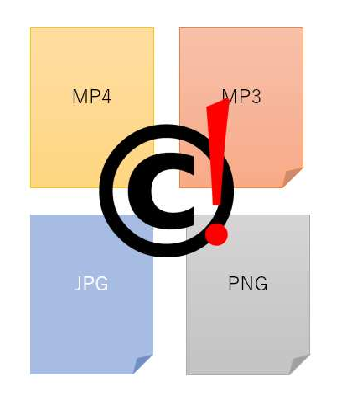
\includegraphics[width=0.25\textwidth]{ome7-img001}
	\item[人を傷つけることや、迷惑になることはやめる]~\\
	インターネットは自分以外の人も使っています。だから、自分勝手なことや悪い言葉を使ってばかりいると人を傷つけたり、\ruby{不快}{ふかい}に思われて犯罪に\ruby{巻}{ま}き\ruby{込}{こ}まれたり、\ruby{訴}{うった}えられたりする可能性もあります。清らかに生きていきましょう。
	\item[他のひとたちが\ruby{困}{こま}らない文字情報を使う]~\\
	ネットワークを使っている人たちはみんな同じものを使っているとは限りません。
	使っている機種が、PCだったり、スマートフォンだったり、ラズベリーパイだったりします。機種によっては、絵文字や特殊文字が見えなくなることが考えられます。
	\item[迷惑メールは見ない、送らない]~\\
	悪い人が色々な都合で出してくる\ruby{怪}{あや}しいメールのことです。。これには、変なアドレスがはられてい
	たり、知らないソフトウェアが貼り付けられたりすることがあります。それを見るとウイルスという悪いものが入ってくることことがあります。ウイルスはコンピュータが\ruby{壊}{こわ}れたり、\ruby{操作}{そうさ}出来なくなったりするものもあります。犯罪者の協力をしたと思われることもあるので、怪しいメールは\ruby{絶対}{ぜったい}に開かないようにしましょう。また、チェーンメール(\ruby{呪}{のろ}いのメールなど)は絶対に信じず他の人に送ってはいけません。
	\item[自分の情報を外に\ruby{漏}{も}らさない]~\\
	自分の名前や、住所などをネットにあげるのはとても\ruby{危}{あぶ}ないから止めましょう。悪い人の目に入ってしまうと家族の身の\ruby{危険}{きけん}にもつながり命の\ruby{保証}{ほしょう}ができません。また、ネットに一度でもあげてしまうと消すことができなくなります。多くの人の目につくからデータが広がってしまうこともあります。ネットにデータをあげるときは問題が無いか\ruby{確認}{かくにん}してからあげましょう。

\end{description}

\clearpage\subsection*{教材を自分のフォルダに置こう}
まずは、今回利用する教材をコピーしましょう。
これまでと同じように、/usr/local/share/ome という場所にあるフォルダ 07をコピーして、/home/ユーザー名 に貼り付けてください。

やり方を忘れてしまった人は、「第1回 4.1 例題1-18 教材をじぶんのフォルダに置こう」 を参考にしてみてください。

\subsection*{1−1インターネットのキホン}
\begin{wrapfigure}{r}[10pt]{0.4\textwidth}
	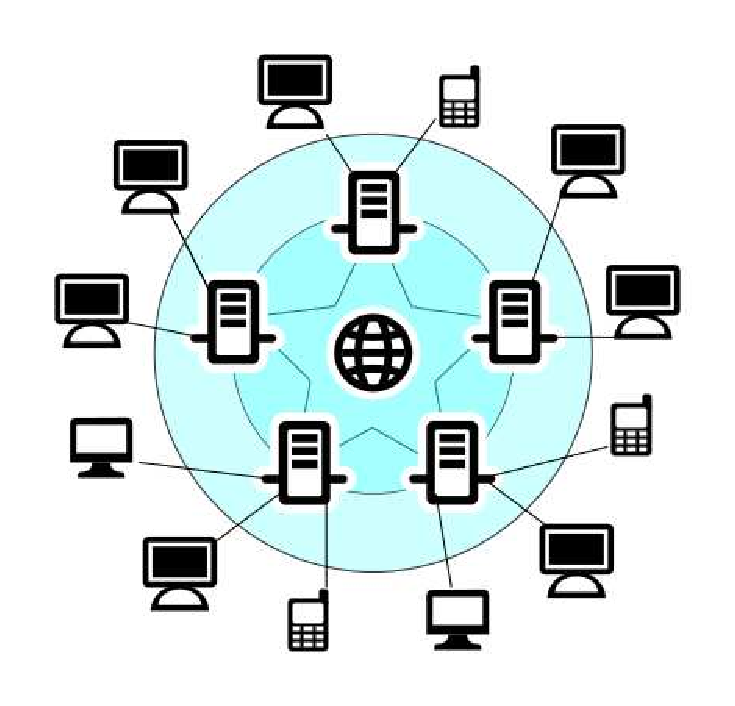
\includegraphics[width=0.4\textwidth]{ome7-img002.eps}
\end{wrapfigure}

みんなが使っているパソコンやスマートフォンなどをたくさんつなぎ、おたがいに情報の\ruby{交換}{こうかん}ができるようにしたものを「ネットワーク」とよんでいます。

インターネットとは、そのネットワークが数えきれないほどのケーブルなどでおたがいにつながりあい、\ruby{網}{あみ}の目のように世界中に広がっているそのもののことです。


\bigskip

みなさんはすでにインターネットを\ruby{触}{さわ}っています。

第一回の\ruby{講義}{こうぎ}でみなさんはwebから画像を自分のラズベリーパイ(PC)に保存しましたね。あれもインターネットを触ったということになるのです。網目のように世界中に広がっているネットワークから好きな画像を調べるということは自分のラズベリーパイでインターネットをしたということになります。

さらに、有名な動画サイト”YouTube”のコンピュータもインターネットにつながっています。そのおかげでインターネットにつながっているパソコンやスマートフォンであればYouTubeの動画を見ることができます。もちろん、インターネットにつながっていなければYouTubeの動画や画像\ruby{検索}{けんさく}など行うことはできません。試しにインターネットを\ruby{切断}{せつだん}してみても面白いかもしれません。


\vfill

\refstepcounter{Question}\theQuestion みんなが使っているパソコンやスマートフォンなどをたくさんつなぎ、おたがいに情報の交換ができるようにしたものを何というでしょうか。




\bigskip

\bigskip

\bigskip

\addBlank{答え}


\bigskip


\bigskip


\bigskip


\bigskip


\clearpage

\subsection*{ 1−2 IPアドレスとは何だろう?}

ネットワークでコンピュータ同士がつながっているときにどうやって通信相手のコンピュータの場所を\ruby{探}{さが}すのでしょうか?

わたしたちのいる住んでいる場所をしめす住所(英語でアドレス)と同じ考え方を使います。
インターネットの住所のことをIP(アイピー)アドレスと言います。
わたしたち日本人は住所を東京都港区高輪2−3−23(東海大学高輪キャンパスの住所)のように表します。
コンピュータの場合は\textbf{数字}で表します。
IPアドレスの場合はxxx.xxx.xxx.xxxのように四つの数字を使って表します。
3ケタづつ「\textbf{.}」点(ドット)で区切ります。
xxxは0~255の数字が入ります。


\bigskip


\centering
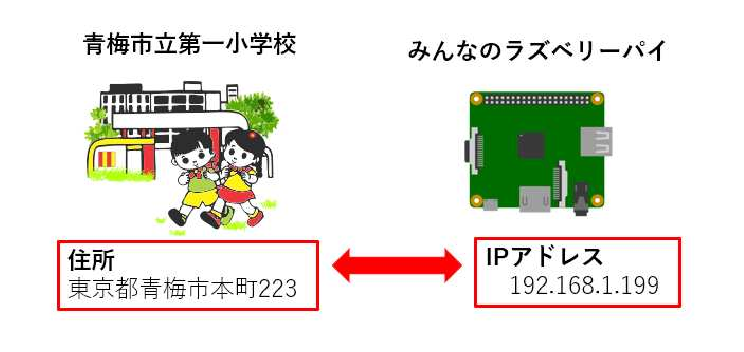
\includegraphics[width=11.024cm]{ome7-img003}


\bigskip


\bigskip


\bigskip





\centering
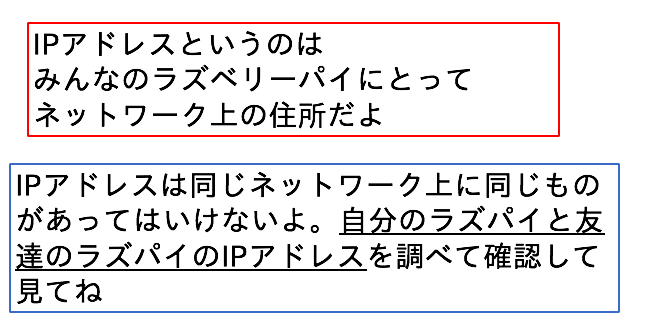
\includegraphics[width=11.412cm]{ome7-img004.png}
\flushleft


\bigskip


\bigskip


\bigskip


\bigskip


\bigskip


\bigskip


\bigskip

IPアドレスはラズベリーパイのネットワーク上の住所に当たるものです。一つのネットワークではIPアドレスは同じものがあってはいけません。例えば、配達する人は同じ住所が世界中にあればどこへ配達したらよいかわからなくなってしまいます。インターネットの場合も同じです。なのでIPアドレスは同じではいけません。ですが、例外として他のローカルIPアドレスでは同じになってしまうことはあります。%\textbf{例題7−1で自分のラズベリーパイのIPアドレスを調べましょう}

\clearpage\subsection*{\bfseries
	1−3 グローバルIPアドレスとローカルIPアドレス}
IPアドレスにはグローバルIPアドレスとローカル(プライベート)IPアドレスという二つに分けられます。



\centering
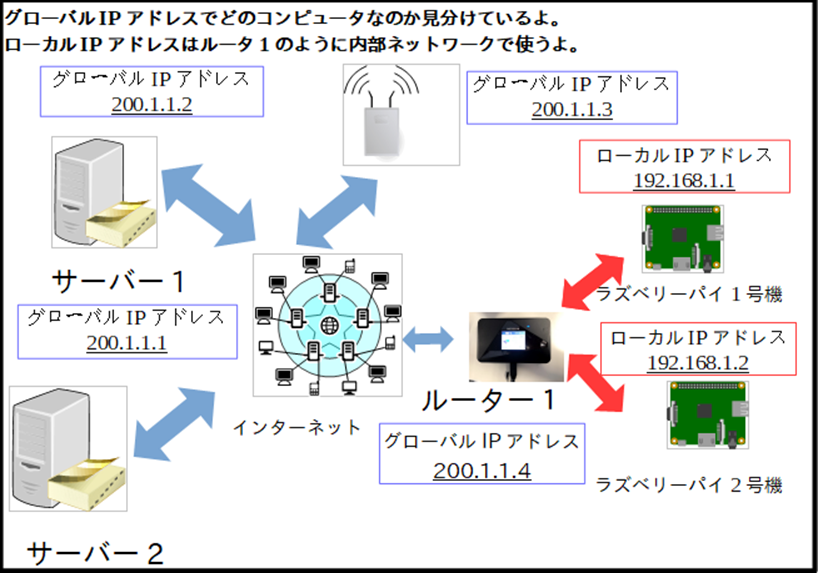
\includegraphics[width=15.0cm]{ome7-img005.png}

\centering
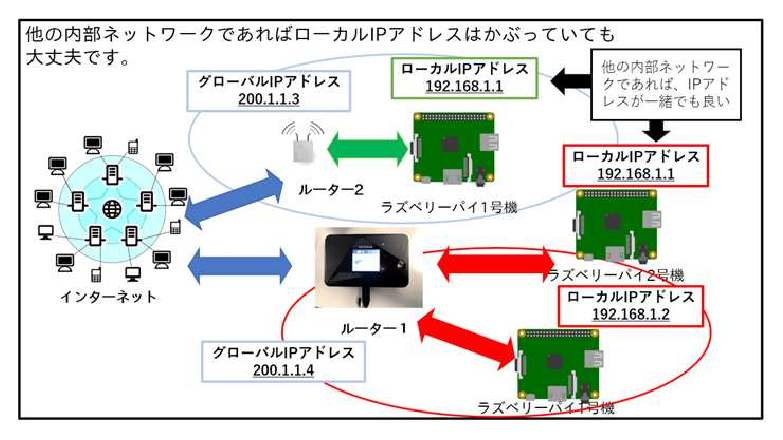
\includegraphics[width=15.0cm]{ome7-img006}
\flushleft

{\refstepcounter{Question}\theQuestion ローカルIPアドレスがかぶっても良いときはどのときですか。}

{\bfseries
	\addBlank{答え}}

	\refstepcounter{Exercise}
\clearpage\subsection*{\theExercise IPアドレスを調べてみよう}
ターミナルにコマンド”hostname
-\texttt{I}”を入力し、自分のラズベリーパイのローカルIPアドレスを確認しよう

{\bfseries
方法}



\centering
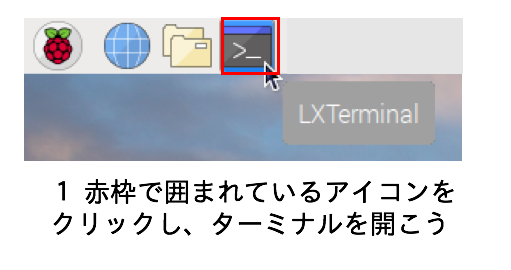
\includegraphics[width=14.566cm]{ome7-img007.png}

\centering
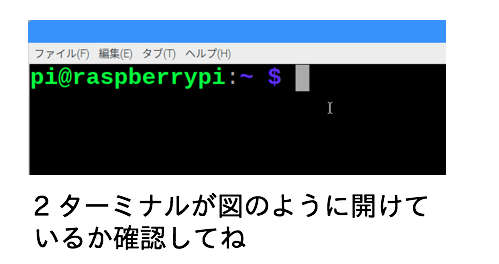
\includegraphics[width=14.52cm]{ome7-img008.png}
\flushleft

\clearpage

\centering

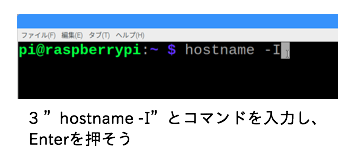
\includegraphics[width=13.799cm]{ome7-img010.png}
\centering
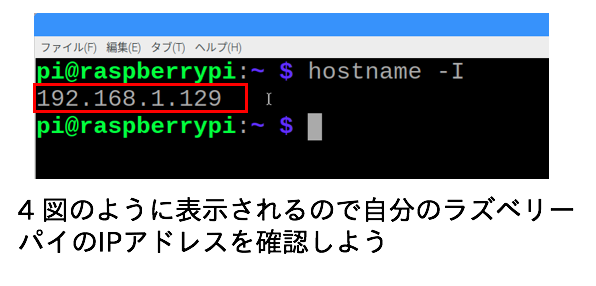
\includegraphics[width=12.771cm]{ome7-img009.png}
\flushleft


\bigskip


\bigskip


\bigskip


\bigskip


\bigskip

{\bfseries
	調べた自分のラズベリーパイのIPアドレスを書こう}

\bigskip


\centering
\begin{tabular}{|p{0.8\textwidth}|} \hline
	\\
	\\
	\\
	\\ \hline
\end{tabular}


\bigskip


\bigskip

\flushleft

{\bfseries
	グループの友達のIPアドレスも教えてもらって書こう}

\bigskip


\centering
\begin{tabular}{|p{0.8\textwidth}|} \hline
	\\
	\\
	\\
	\\ \hline
\end{tabular}


\flushleft


\subsection*{\bfseries }
\clearpage
\textbf{1−4 インターネットのつながりについて知ろう}

教室内では無線通信を利用してインターネットを使用しています。第1回目の授業の最初に\ruby{皆}{みな}さんはインターネット\ruby{接続}{せつぞく}をしました。\ruby{実際}{じっさい}にはどこにつながっているかというと下の図のルータです。

\centering
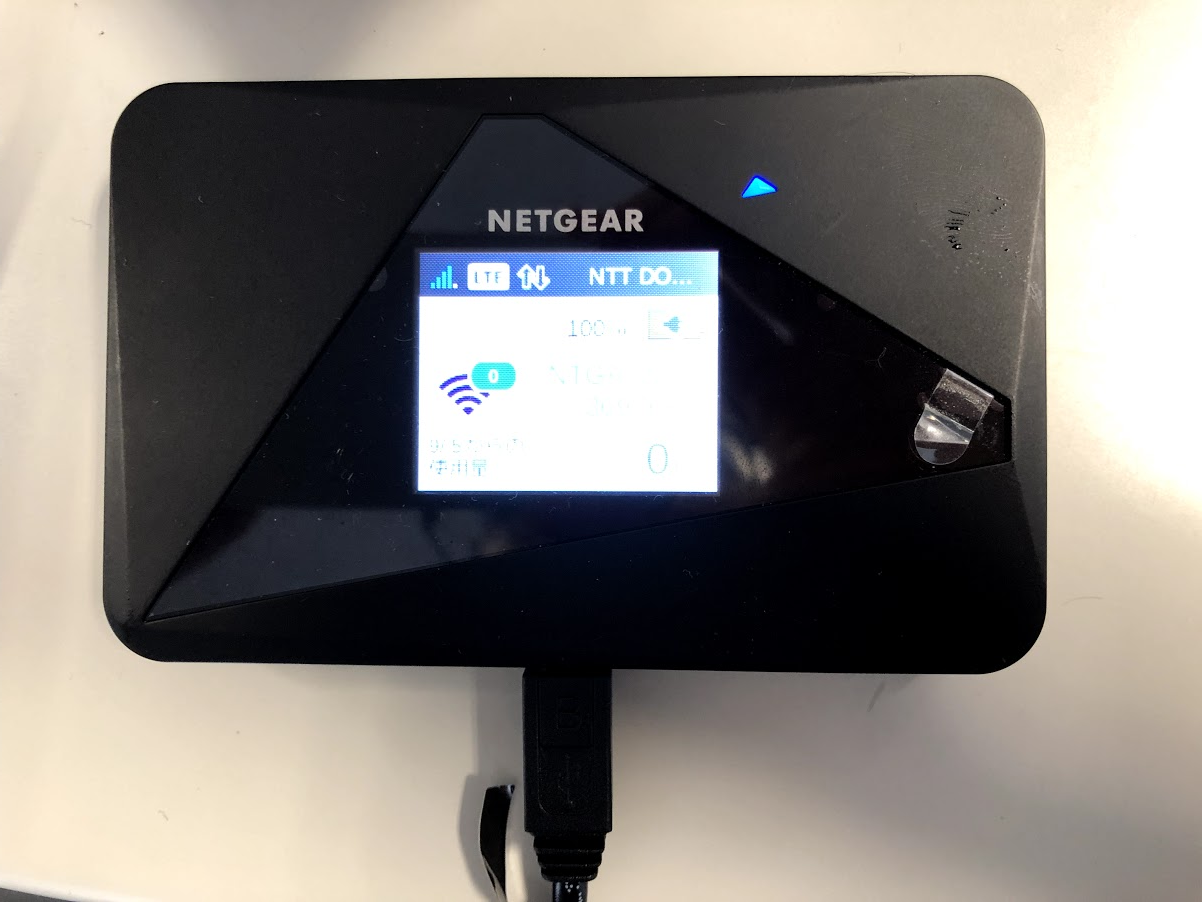
\includegraphics[width=8.186cm]{ome7-img011.png}
\flushleft


\bigskip


\bigskip


\bigskip


\bigskip


\bigskip


\bigskip


\bigskip


\bigskip

この機械のおかげで、みんなは教室内でインターネットをすることができているんだ。

どういう原理で、みんなのラズベリーパイでインターネットを使用できているか説明していくよ。

みんなのラズベリーパイは直接インターネットにつながってはいません。一度、ルータを経由しています。このルータのおかげで\ruby{複数}{ふくすう}のラズベリーパイやPCを同時にインターネットにアクセスさせることができるんだ。以下の図がイメージ図だよ。


\bigskip



\centering
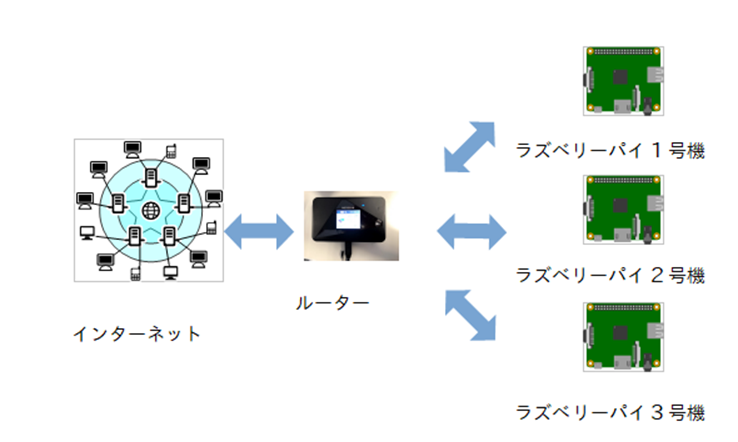
\includegraphics[width=15.214cm]{ome7-img012.png}
\flushleft


\bigskip

ではどのようにして複数台のラズベリーパイをインターネットに接続しているのでしょうか。それはルータに\textbf{グローバルIPアドレス}というものを\ruby{割}{わ}り当てて、ルータが他のラズベリーパイの代表として通信を行っています。どういうことかわかりずらいので、図でみていきましょう。



\centering
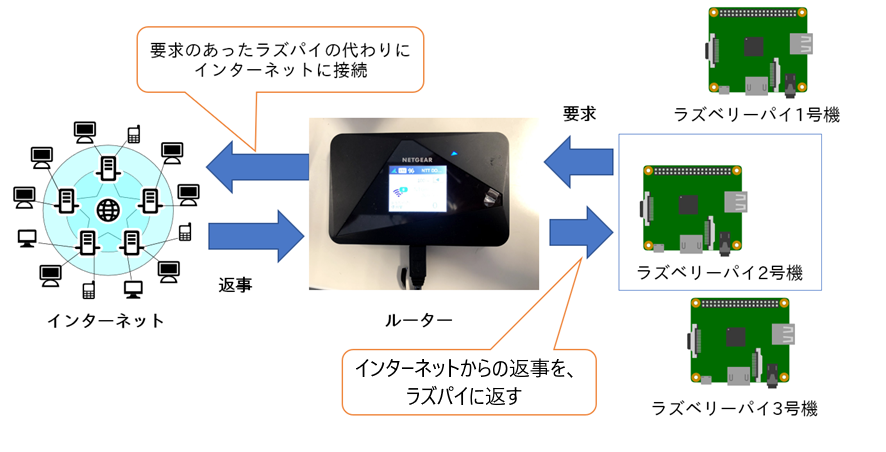
\includegraphics[width=16.18cm]{ome7-img013.png}
\flushleft


\bigskip

図ではラズベリーパイ2号機がインターネットにアクセスし、何かしらの webサイトを観たいと要求したとします。その要求はまずルータのところにいき、ラズベリーパイ2号機の代わりにインターネットに接続します。その接続で、ルータはインターネット先から返事をもらい、そのインターネットからの返事をラズパイに返しています。

\centering
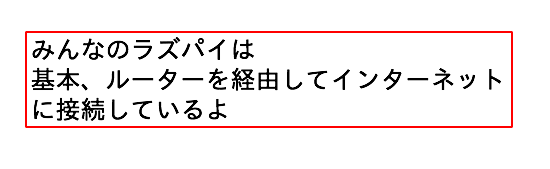
\includegraphics[width=15.921cm]{ome7-img014.png}
\flushleft


\bigskip

\clearpage
これだけではうまくいかないことがあります。下の図をみてください。



\centering
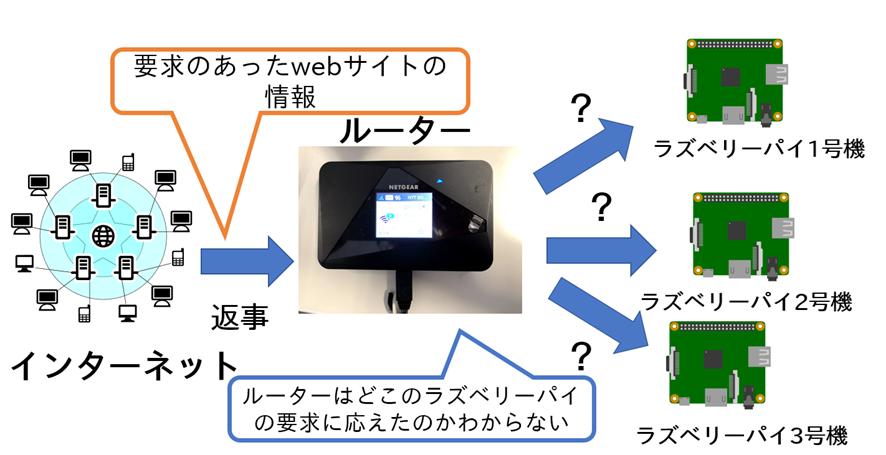
\includegraphics[width=15.565cm]{ome7-img015.png}
\flushleft

どれかしらのラズベリーパイからwebサイトへの要求があり、ルータを経由してインターネットに接続します。そのあと、インターネットから要求のあったwebサイトの情報がルータにいきます。ここで問題が発生します。それはいったいのどのラズベリーパイの要求であったのかルータがわからないのです。\ruby{僕}{ぼく}らが、勝手にラズベリーパイ1号機、ラズベリーパイ2号機、ラズベリーパイ3号機と名前をつけて\ruby{判断}{はんだん}していても、そのことはルータはわかりません。そこでIPアドレスというものを使います。

ルータは自分を\ruby{含}{ふく}め、ローカルIPアドレスを割り当てています。このローカルIPアドレスでラズベリーパイを見分けています。
%\textbf{例題7−2で自分のラズベリーパイが接続しているグローバルIPアドレスを確認してみよう}

\bigskip

\centering
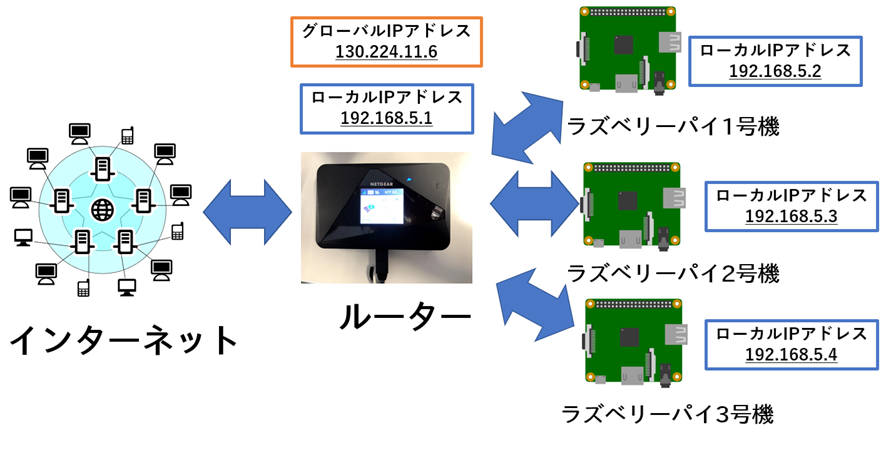
\includegraphics[width=14.233cm]{ome7-img016.png}
\flushleft


\bigskip

\refstepcounter{Question}\theQuestion ルータはラズベリーパイたちを見分けるために何を割り当てていますか。

\bigskip


\bigskip
\addBlank{答え}

\refstepcounter{Exercise}
\clearpage\subsection*{\theExercise ポケットWi-FiルータのグローバルIPアドレスを調べよう}
\begin{minipage}[b]{0.58\textwidth}
	ターミナルを開き、”curl

	inet-ip.info”とコマンドを入力して、自分のラズベリーパイが接続しているwifiルータのグローバルIPアドレスを確認しよう

	curlコマンドはインターネットから情報を取ってくるときに使用します。今回は”inet-ip.info”というサイトからグローバルIPアドレスを調べてターミナルに\ruby{表示}{ひょうじ}させています。webブラウザから”inet-ip.info”にアクセスしてみると右の図のような形でグローバルIPアドレスを確認することもできます。

\end{minipage}
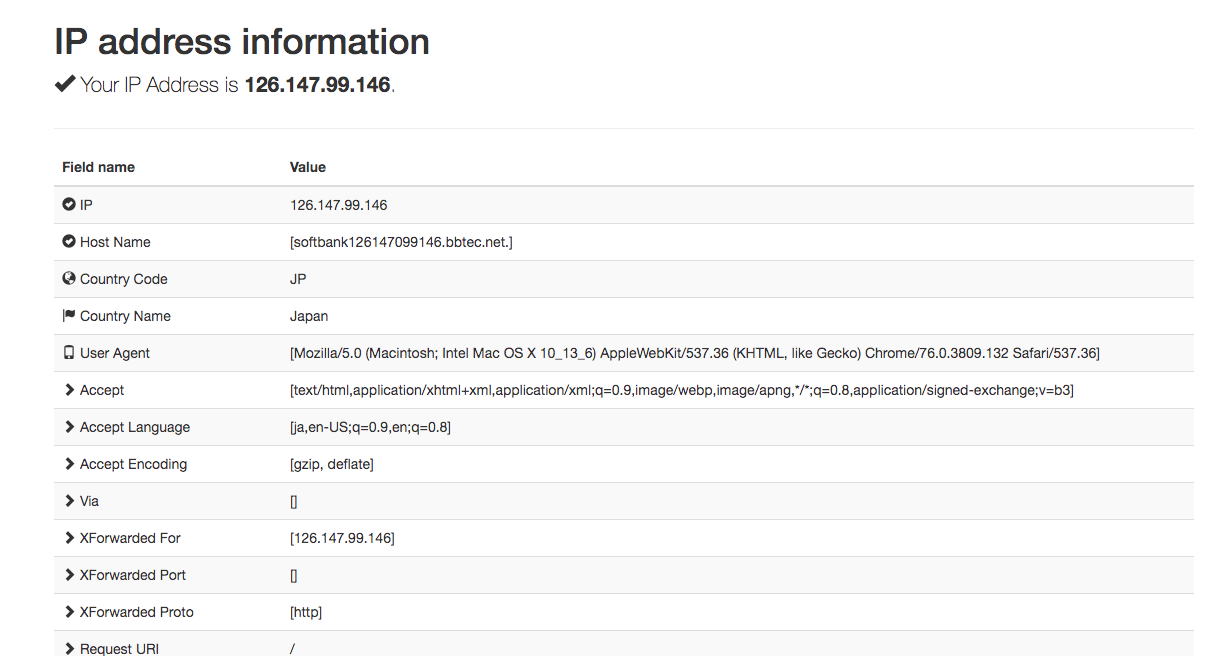
\includegraphics[width=0.4\textwidth]{ome7-img017.png}



\bigskip

{\bfseries
	方法}



\centering
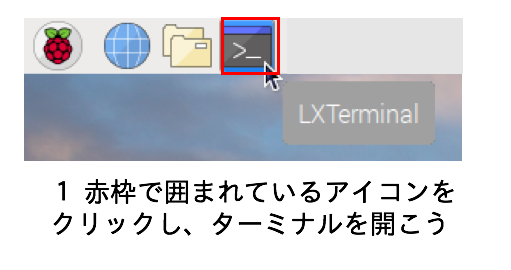
\includegraphics[width=13.942cm]{ome7-img007.png}

\centering
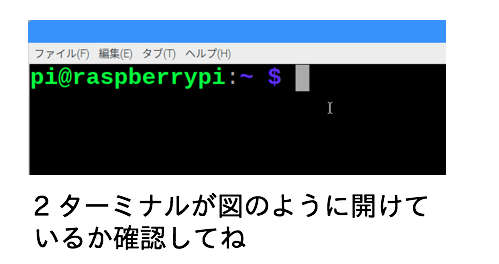
\includegraphics[width=12.746cm]{ome7-img008.png}
\flushleft


\bigskip


\bigskip


\bigskip


\bigskip



\centering
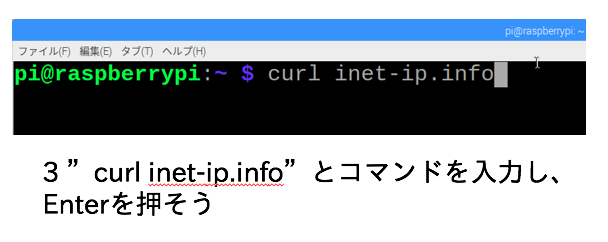
\includegraphics[width=13.716cm]{ome7-img018.png}

\centering
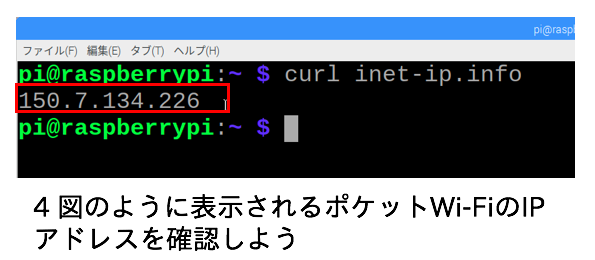
\includegraphics[width=13.85cm]{ome7-img019.png}
\flushleft


\bigskip


\bigskip

{\bfseries
	調べたグローバルIPアドレスを書こう}


\bigskip


\centering
\begin{tabular}{|p{0.8\textwidth}|} \hline
	\\
	\\
	\\
	\\ \hline
\end{tabular}


\flushleft




\bigskip


\bigskip

{\bfseries
	グループの友達がしらべたポケットWi-FiのIPアドレスも教えてもらって書こう}



\bigskip


\centering
\begin{tabular}{|p{0.8\textwidth}|} \hline
	\\
	\\
	\\
	\\ \hline
\end{tabular}


\flushleft



\bigskip


\bigskip

\clearpage\subsection*{1−5 ポート番号とは}


\centering
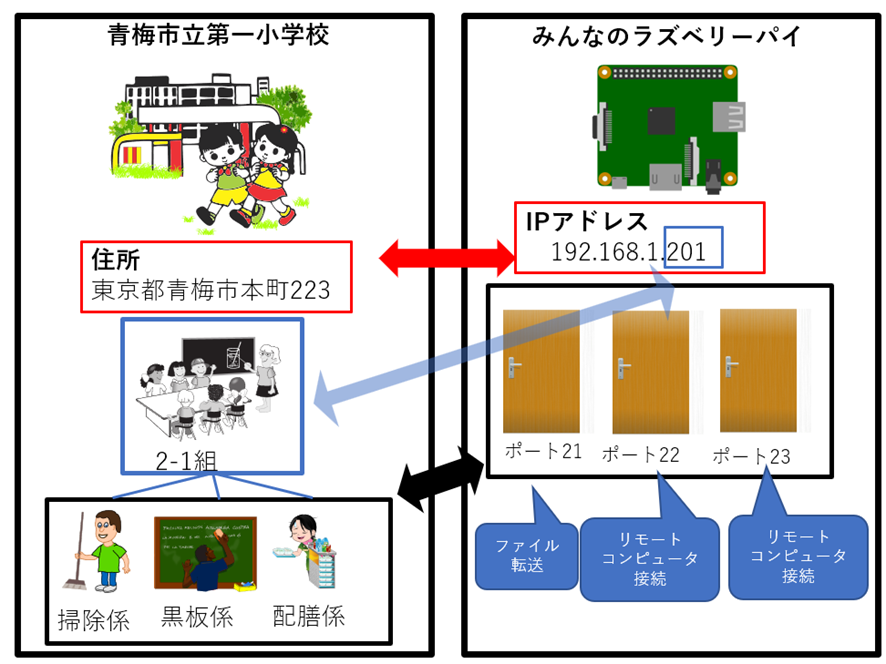
\includegraphics[width=15.004cm]{ome7-img020.png}
\flushleft

前のページではみんなはラズベリーパイがどのようにインターネットにつながっているのか理解してくれたと思います。
ここではさらにポート番号について\ruby{知識}{ちしき}を深めましょう。
IPアドレスでは通信相手となる別のネットワークのコンピュータを特定することができます。
しかし、コンピュータでは\ruby{通常}{つうじょう}、多くのプログラム(機能)が動作していて、IPアドレスを指定するだけでは、どのプログラムと接続するかを区別できません。
そこでコンピュータ上の、\underline{どのプログラムと接続するかを指定するためにポート番号が用いられます}。
下の図は小学校を例にしています。

青梅市立第一小学校の住所がみんなのラズベリーパイのIPアドレスに\ruby{対応}{たいおう}しており、IPアドレスの\ruby{末尾}{まつび}の201(青で囲まれている)が小学校のクラスに対応しています。
皆さんの学校でも生徒にはそれぞれ係という役割が\ruby{与}{あた}えられていますね。
例えば、プリントなどの\ruby{配布物}{はいふぶつ}を配る配り係、黒板を使い終わったらきれいにする黒板係、教室の\ruby{窓}{まど}をきれいにする窓ふき係などこれらの係に相当するものがラズベリーパイにもあり、それが\underline{ポート}です。
ポート21はファイル転送用の働きをする\ruby{担当}{たんとう}で、ポート22と23は他のコンピュータに接続する担当です。
ポートには役割がありインターネットの通信はファイル転送であったり、他のコンピュータに接続して\ruby{遠隔}{えんかく}操作したり、webページにアクセスしたりといろいろあります。
なので、その分のポートを用意しておき、役割を与え、対応している役割のときに\ruby{頑張}{がんば}ってもらう仕組みになっています。
みんなのラズベリーパイやパソコン、サーバにはポートは何個あるのか調べてみるのも面白いですね。

\bigskip


\refstepcounter{Question}\theQuestion ポート番号はどのようなことに使われますか。
\bigskip

\addBlank{答え}


\clearpage

ここでは実際にポートはネットワーク上ではどのように使うのか、下の図を見てみましょう。



\centering
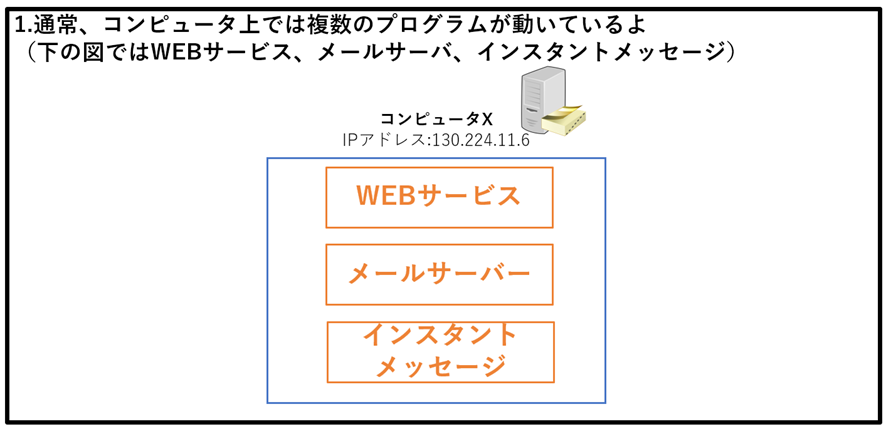
\includegraphics[width=16.609cm]{ome7-img021.png}

\centering
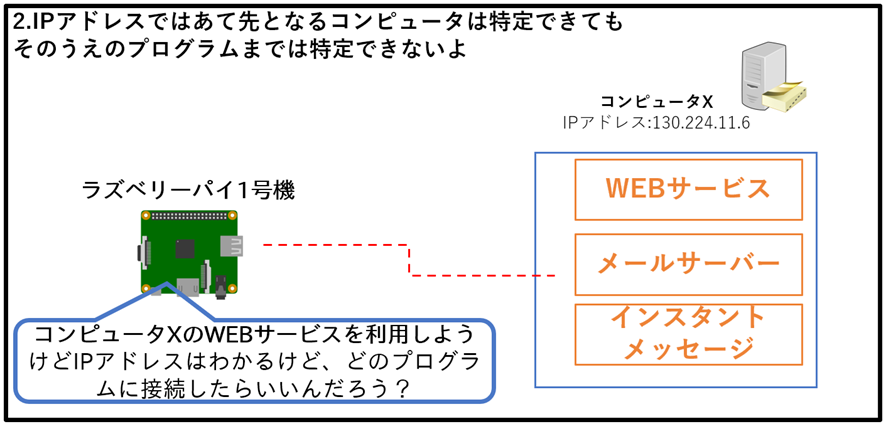
\includegraphics[width=16.496cm]{ome7-img022.png}
\flushleft


\bigskip

\clearpage

\centering
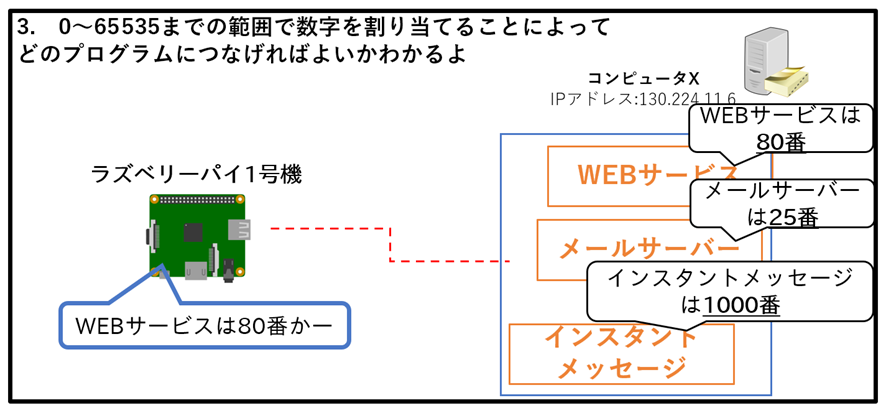
\includegraphics[width=16.843cm]{ome7-img023.png}



\centering
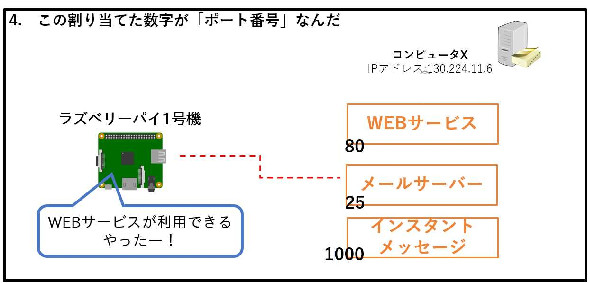
\includegraphics[width=16.875cm]{ome7-img024}
\flushleft


\bigskip


\bigskip


\bigskip

さらにラズベリーパイ側のポートはラズベリーパイが自動で割当ており、そこからデータを受け取っているよ。


\bigskip


\bigskip


\bigskip



\centering
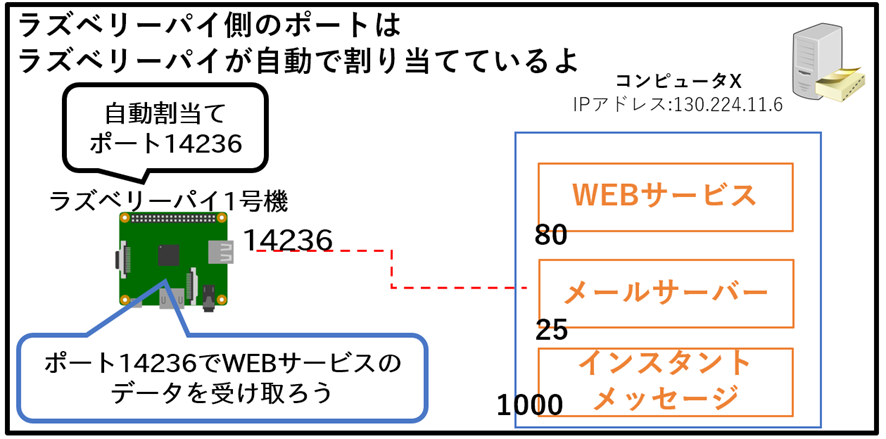
\includegraphics[width=15.847cm]{ome7-img025.png}
\flushleft

コンピュータXのようにネット上にサービスを\ruby{提供}{ていきょう}するコンピュータを\underline{サーバ}と言います。

ラズベリーパイ1号機のようにサーバからサービスを受けるコンピュータを\underline{クライアント}言います。


\bigskip

これらのポートが今\ruby{現在}{げんざい}どのようなことに使われているのか\textbf{例題7−3で確認してみましょう。}


\bigskip

{\refstepcounter{Question}\theQuestion コンピュータ上のプログラムを判断するためになにが用いられていますか。}
\bigskip

{\bfseries
	\addBlank{答え}}

\bigskip
\bigskip
{\bfseries
	ネット上にサービスを提供するコンピュータとネット上のコンピュータからサービスを受けるコンピュータをそれぞれ何といいますか。}

\bigskip
\bigskip
{\bfseries
	\addBlank{答え}}


\bigskip


\bigskip


\bigskip

\clearpage\subsection*{1−6 DNS(Domain Name System)について}

{\bfseries
	IPアドレスは住所であり、それがわからないとサーバのサービスをうけることはできません。ですが以下の図のようなことが起こることがあります。}

\centering
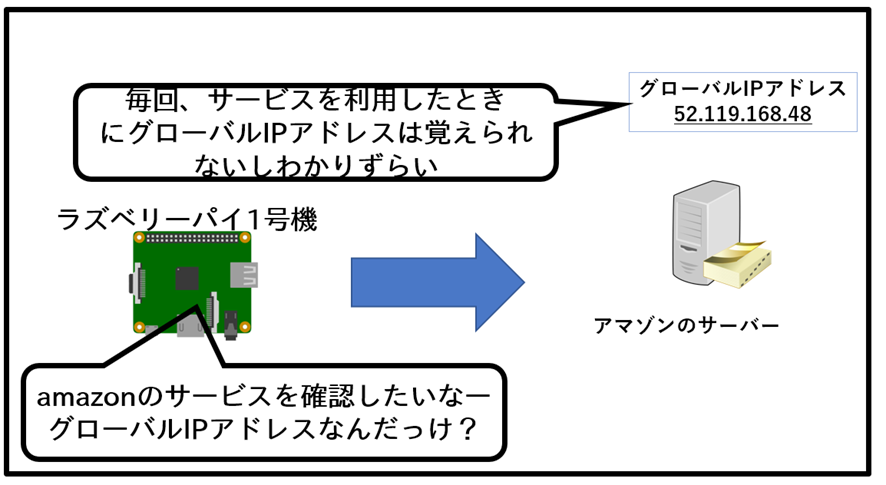
\includegraphics[width=15.004cm]{ome7-img026.png}
\flushleft

そこで、DNSサーバと言うものを作り、一度そこに”amazon.co.jp”のグローバルIPアドレスを教えてもらってサーバに接続しています。



\centering
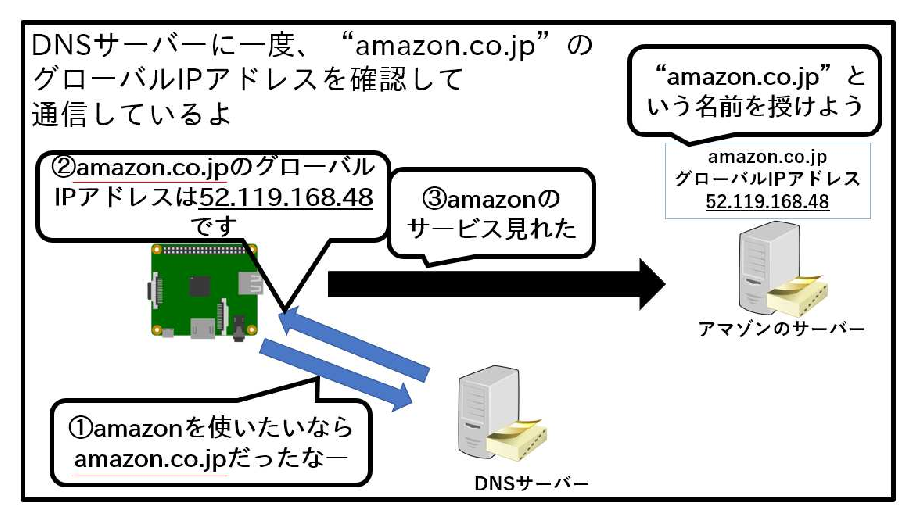
\includegraphics[width=13.051cm]{ome7-img027}
\flushleft



\bigskip

\clearpage

\centering
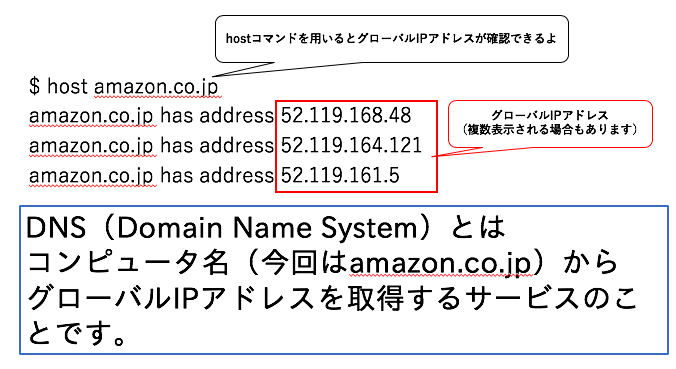
\includegraphics[width=11.924cm]{ome7-img028.png}
\flushleft


\bigskip


\bigskip

{\refstepcounter{Question}\theQuestion ターミナルを開き、”host
	amazon.co.jp”を実行してグローバルIPアドレスを確認しよう。}

\bigskip
{\bfseries
	\addBlank{答え}}

\clearpage\subsection*{\bfseries コラム NATについて}

教科書の前のページでローカルIPアドレスとグローバルIPアドレスが存在することを皆さんは知りましたね。ここではもっと細かくIPアドレスを用いたインターネット接続を勉強しましょう。インターネットに接続するコンピュータは自分自身を示すIPアドレスとして世界で\ruby{唯一}{ゆいつ}のグローバルIPアドレスを使わなければならないのです。みなさんのラズベリーパイにはローカルIPアドレスしか割り当てられていませんので、このままではインターネットをすることはできません。そこでNAT(Network
Address
Translation)というものを用います。このNATはルータが行っていて、送信元のローカルIPアドレスをグローバルIPアドレスに変換して通信を行っています。具体的にはどのようになっているのか下の図をみて確認してみよう。



\centering
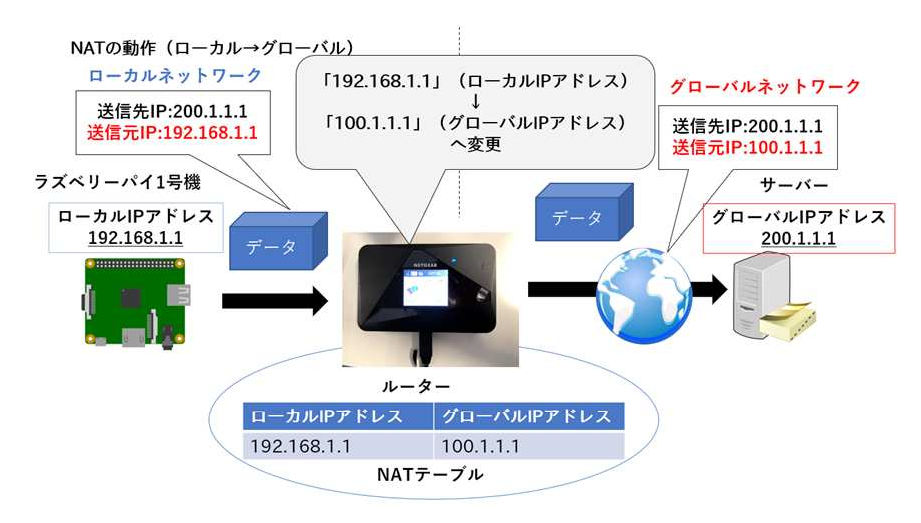
\includegraphics[width=11.352cm]{ome7-img029}
\flushleft


\bigskip



ラズベリーパイ1号機からサーバにデータの送信先IPアドレスは200.1.1.1(グローバルIPアドレス)、送信元IPアドレスは192.168.1.1(ローカルIPアドレス)です。NATを行うルータは、プライベートアドレスとグローバルアドレスの\ruby{境界}{きょうかい}に位置しています。ここでルータは、ラズベリーパイから送信されたデータの送信元IPアドレス192.168.1.1を、グローバルIPアドレスの「100.1.1.1」に変換して転送します。このときルータは、その変換情報をNATテーブルに記録しています。この記録が、「返ってくるデータ」、つまりサーバーからラズベリーパイへ送られるデータの転送時に役立ちます。次の図を見てください。



\centering
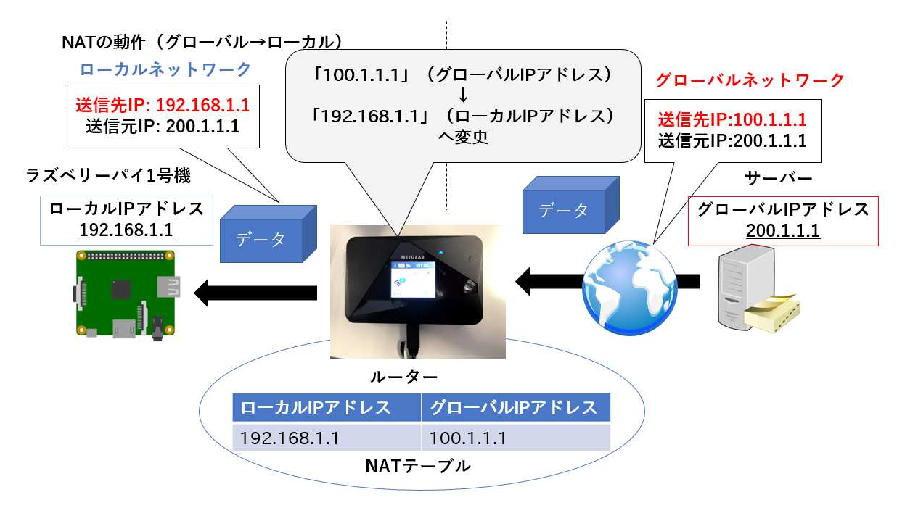
\includegraphics[width=10.83cm]{ome7-img030}
\flushleft



\bigskip

サーバーからラズベリーパイへの返事のデータの送信先IPアドレスは「100.1.1.1」、送信元IPアドレス「200.1.1.1」になりますね。データがルータへ転送されてくると、ルータはNATテーブルを確認して、送信元IPアドレスを「100.1.1.1」から元の「192.168.1.1」へ変換します。これにより返りのデータの通信が可能になるのです。NATによって送信元のローカルIPアドレスをグローバルIPアドレスに変換して通信をおこなっているおかげでみんなはインターネットを利用できているんだね。


\bigskip


\bigskip

\refstepcounter{Exercise}
\clearpage\subsection*{\theExercise 開いているポートを調べてみよう}
ターミナルを開き、”nmap
localhost”とコマンドを入力し、ポートについて知ろう

{\bfseries
方法}



\centering
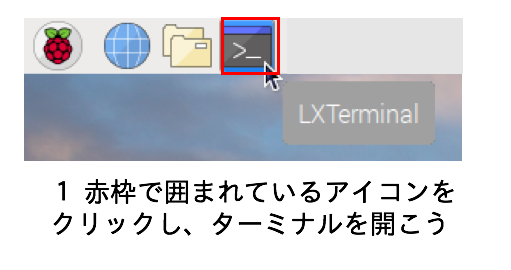
\includegraphics[width=14.981cm]{ome7-img007.png}

\centering
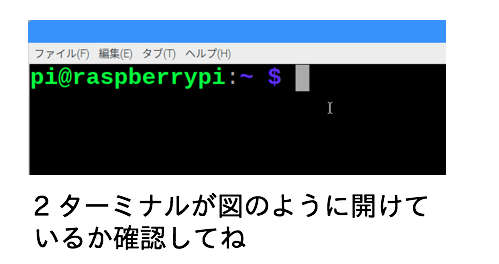
\includegraphics[width=14.508cm]{ome7-img008.png}
\flushleft


\clearpage





\centering

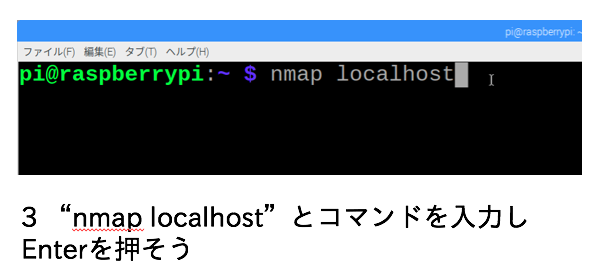
\includegraphics[width=14.404cm]{ome7-img032.png}
\bigskip
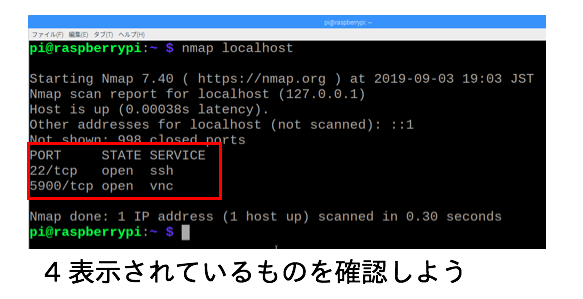
\includegraphics[width=14.542cm]{ome7-img031.png}
\flushleft

\bigskip
{\bfseries
	自分のラズベリーパイに表示されたものを下の表に書こう}

\begin{flushleft}
	\tablefirsthead{}
	\tablehead{}
	\tabletail{}
	\tablelasttail{}
	\begin{supertabular}{|m{5.467cm}|m{5.4690003cm}|m{5.155cm}|}
		\hline
		PORT &
		STATE &
		SERVICE\\\hline
		~
		&
		~
		&
		~
		\\\hline
		~
		&
		~
		&
		~
		\\\hline
		~
		&
		~
		&
		~
		\\\hline
		~
		&
		~
		&
		~
		\\\hline
	\end{supertabular}
\end{flushleft}
{\bfseries
serviceに出てきた言葉をインターネットを使って調べよう。
皆さんにとっては\ruby{難}{むず}しい言葉が多いと思います。
それでも自分で調べてみましょう。
それが知識を深める近道です。\\
ポートが開いていない場合、コマンドは何も表示せず、
改行が起こるだけのこともあります。
}

\clearpage\subsection*{2−1 HTMLについて}
\refstepcounter{Exercise}
\subsection*{\theExercise HTMLの復習}
{\bfseries
	考え方\newline

	第1回で作成した\ruby{自己紹介}{じこしょうかい}ページのタグや機能を理解することでHTMLについて自分の思ったとおりに作れるようになりましょう。}


\bigskip

HTMLは、タグという一つの機能をつかい、ウェブページを作り出します。\newline
タグというのは、{\textless}{\textgreater}{\textless}/{\textgreater}という形です。見覚えのある形ですね。\newline
例えば、

\ \ {\textless}p{\textgreater}文章をここに書きます。{\textless}/p{\textgreater}

のようなタグをpタグと\ruby{呼}{よ}びます。pタグはタグの間にある文章を表示します。\newline
まずは、第1回目の授業でみさなんが作成した自己紹介ページとその画像のファイルを第6回のフォルダにコピーし、それをmousepadでhtmlファイルを開いて見ましょう。

\begin{minipage}[b]{0.5\textwidth}
	\begin{enumerate}
		\begin{minipage}[b]{1.5\textwidth}
			\item \ \ cp \ \ {\textasciitilde}/01/self\_intro.html \ \ \ {\textasciitilde}/07/www/index.html\\
			cpコマンドを使って、 自己紹介ページのhtmlと<img src="face.png" などimgタグで指定している画像ファイルを、 第7回のwwwディレクトリにコピーしましょう。\\
			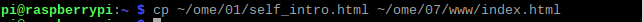
\includegraphics[width=14.73cm]{ome7-img033.png}
		\end{minipage}

		\bigskip

		\item

		      \ \ cd \ \ {\textasciitilde}/07/www/\newline
		      cdコマンドを使って、(cpコマンドとは\ruby{違}{ちが}うよ。) 第7回のwwwディレクトリに\ruby{移動}{いどう}。


		\item \ \ mousepad\ \index.html

		      \ \ mousepadでコピーした自己紹介のhtmlを開いてみよう。

	\end{enumerate}
\end{minipage}
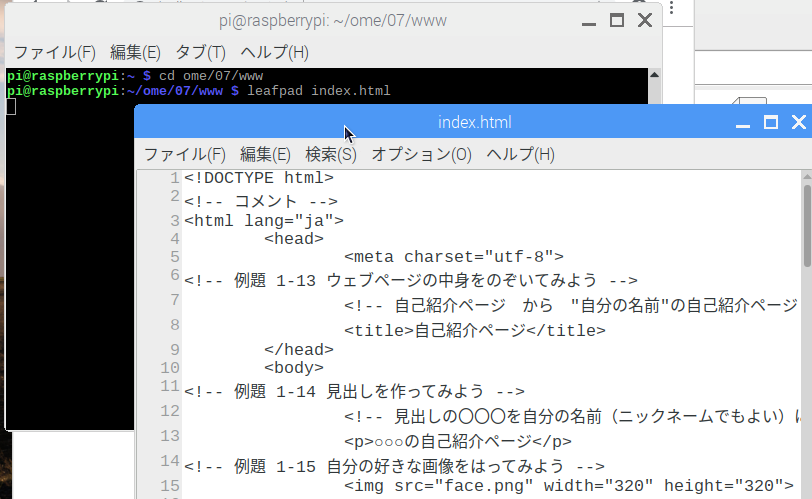
\includegraphics[width=0.45\textwidth]{ome7-img034.png}

\bigskip

開いたhtmlファイルの中に、実際にはウェブページに出てこない文章がちらほら見えます。

\ \ \ \ \ \ {\textless}!-{}- コメント -{}-{\textgreater}

それは、コメントという機能でウェブページには表示されない、メモのような機能でプログラムを書くときにあると便利です。HTMLに限らずHSPや様々なプログラム言語、はたまた現実世界でもメモというのは大切なので必要な情報はしっかりと書いておきましょう。

self\_intro.html内に使われたタグをまとめました。これを参考に自己紹介ページをより良くしていきましょう。

\clearpage
HTMLまとめ\ \

\begin{center}
	\tablefirsthead{}
	\tablehead{}
	\tabletail{}
	\tablelasttail{}
	\begin{supertabular}{|m{4.0cm}|m{12.0cm}|}
		\hline
		タグ名 &

		\ruby{効果}{こうか}\\\hline

		{\textless}title{\textgreater}{\textless}/title{\textgreater} &
		ウェブページのタイトルをつける\\\hline
		{\textless}h1{\textgreater}{\textless}/h1{\textgreater} &
		見出し(h1~h6)まで使える。h1が一番大きい\\\hline
		{\textless}ul{\textgreater}{\textless}/ul{\textgreater} &

		点付のリスト。リストの\ruby{項目}{こうもく}はliを使って表す\\\hline
		{\textless}li{\textgreater}{\textless}/li{\textgreater} &
		リストの項目。ulもしくはolタグなどの中で使う\\\hline
		{\textless}p{\textgreater}{\textless}/p{\textgreater} &
		\ruby{段落}{だんらく}を作るために使う。文字を表示したいときはこれを使う。改行は自動で行われるので自分のタイミングで行いたいときは{\textless}br{\textgreater}を使う\\\hline
		{\textless}br{\textgreater} &
		改行. pの中でも使うことができる\\\hline
		{\textless}i{\textgreater}{\textless}/i{\textgreater} &
		イタリック(少し\ruby{傾}{かたむ}いた感じの文字)\\\hline
		{\textless}u{\textgreater}{\textless}/u{\textgreater} &
		文字の下に線を引くときに使う\\\hline
		{\textless}a href=””{\textgreater}{\textless}/a{\textgreater} &
		リンクを貼りたいときに使う。hrefにはクリックしたときに飛びたいURLを入れる。\\\hline
		{\textless}img src=””{\textgreater} &
		画像を表示するときに使用する。srcには画像の場所を指定する。ラズベリーパイの中の画像を指定しても、URLとして指定しても良い。\\\hline
		{\textless}ol{\textgreater}{\textless}/ol{\textgreater} &
		番号付きのリスト.
		liでリストの項目を決める。

		番号はliの書いた順番通りになる\\\hline
	\end{supertabular}
\end{center}

\bigskip

HTMLで使いたい色を探すときにはここを使うと便利です。

\url{https://www.colordic.org/m/}\newline
地下鉄のシンボルカラーとカラーコードで使いたい色がわかるはずです。

\url{https://www.colordic.org/}\newline
色の名前とカラーコードがわかります。色がまんべんなくあります。

\url{https://tech-unlimited.com/color.html}\newline
上級者向け、色の三原色というものから実際にHTML用のカラーコードに変えるサイトです。

\clearpage
また、HTMLにはボタンや文字を書き込む部分も作れます。\newline
通常見るだけのウェブページだったものがデータの送受信を可能とするなど、可能性を広げられます。

一部のタグを下に\ruby{記載}{きさい}します。

\begin{center}
	\tablefirsthead{}
	\tablehead{}
	\tabletail{}
	\tablelasttail{}
	\begin{supertabular}{|m{8.6cm}|m{7.91cm}|}
		\hline
		{\textless}form{\textgreater}{\textless}/form{\textgreater}

		(使用例)

		\ {\textless}form action=”cgi-bin/formmail.cgi” {\textgreater} &
		入力送信フォームを作成

		formタグの中に
		{\textless}input{\textgreater},
		{\textless}select{\textgreater},
		{\textless}textarea{\textgreater}
		などをいれることで

		ボタンや文字入力欄を作れる\\\hline
		{\textless}input{\textgreater}{\textless}/input{\textgreater}

		(使用例)

		{\textless}input type=”password” name=”pass”{\textgreater} &
		文字の入力や、ボタンなどを作成するタグ。


		inputの次にtypeなどの\ruby{属性}{ぞくせい}を入れることで一行の文章やパスワードの入力などを決定する\\\hline
	\end{supertabular}
\end{center}

\bigskip

それでは、formを使った例題を説いてみましょう。

例題\newline
自己紹介ページの一番下から2行上あたりにある{\textless}/body{\textgreater}の上の行から{\textless}form{\textgreater}タグで文字の入力をし、送信ボタンを\ruby{押}{お}せる機能を書きましょう。

考え方\newline
はじめに、formタグの間({\textless}form{\textgreater}
**ここ**{\textless}/form{\textgreater})に、inputタグでテキストボックスを作る。そして、同じようにinputタグを使って送信ボタンという名前のボタンを作成する。

1.{\textless}form{\textgreater}{\textless}/form{\textgreater}を書き込めるスペースを作ろう。



\centering
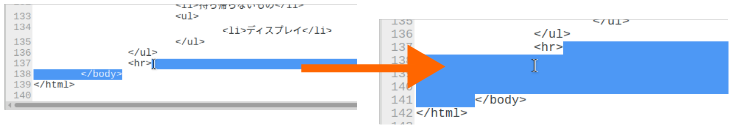
\includegraphics[width=17.006cm]{ome7-img035.png}
\flushleft

2.{\textless}form{\textgreater}タグを書き足そう。



\centering
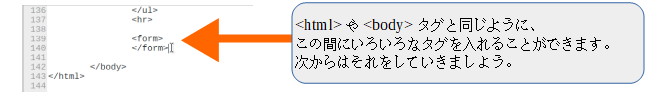
\includegraphics[width=17.006cm]{ome7-img036.png}
\flushleft


\bigskip


\bigskip

3.{\textless}form{\textgreater}タグの間に、行を作り「テキストボックス」という文字が出るようにしよう。\newline
\ \ {\textless}form{\textgreater}\newline
\ \ \ \ \textbf{\textit{{\textless}p{\textgreater}テキストボックス{\textless}/p{\textgreater}}}\newline
\ \ {\textless}/form{\textgreater}

4.次の行に{\textless}input{\textgreater}タグを入れよう。その際に、テキストを書き込めるようにしよう。

%\newline
\ \ 画像のようにするためには、\newline
\ \ {\textless}form{\textgreater}\newline
\ \ \ \ {\textless}p{\textgreater}テキストボックス{\textless}/p{\textgreater}\newline
\ \ \ \ \textbf{\textit{{\textless}input \ \ type=”text” \ \ size=”10”{\textgreater}}}\newline
\ \ {\textless}/form{\textgreater}

\centering
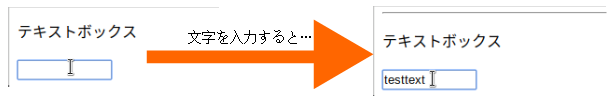
\includegraphics[width=16.3cm]{ome7-img037.png}
\flushleft

5.同じようなやり方で、先にかいた{\textless}input{\textgreater}タグから改行して次の行に{\textless}input{\textgreater}タグで送信ボタンを作成しよう。\newline
\ \ \ \ \textbf{\textit{{\textless}input type=”submit” value=”送信”{\textgreater}}}

6.作成したHTMLファイルを保存し、実際にブラウザで作成されているか確認してみましょう。\newline


このように、formタグ、inputタグには便利な機能があります。\newline
以下に、inputタグの属性を一部記載しておきますので、\textbf{参考にして}問題を解いていきましょう。


\bigskip

\clearpage
\refstepcounter{Question}\theQuestion\newline
\begin{enumerate}
	\item 最初に書いたテキストボックスの属性をパスワード入力ボックスに書き換えてみよう。
	\item 食べ物の名前を{\textless}p{\textgreater}タグを使って3つ追加してその横にチェックボックスを置きましょう。
	\item リセットボタンを送信ボタンの次の行に追加してみよう。
\end{enumerate}

\samepage

わからなかったら、先生に質問をすること。その間は\ruby{一覧}{いちらん}を見て考えてみよう。

inputタグの機能になるもの

\begin{flushleft}
	\tablefirsthead{}
	\tablehead{}
	\tabletail{}
	\tablelasttail{}
	\begin{supertabular}{|m{3.4459999cm}|m{7.9160004cm}|}
		\hline
		type=”text” &
		1行のテキストボックスを作ります。\newline
		sizeの属性を指定することで大きさも決定できる。\\\hline
		type=”password” &
		パスワード用のテキストボックスを作ります。\newline

		入力されたら*のマークなどに置き換わります。送信する際には\ruby{普通}{ふつう}の文字で送られるのに注意。\\\hline
		type=”checkbox” &
		チェックボックスを作ります。
		複数\ruby{選択}{せんたく}可能で、checked属性を指定すると予めチェックが入ったかどうかを決めれる。\\\hline
		type=”radio” &
		ラジオボタンを作ります。
		複数の中から1つしか選択できないのが\ruby{特徴}{とくちょう}。\newline
		こちらもcheckedで\ruby{状態}{じょうたい}を決めれる。\\\hline
		type=”submit” &
		送信ボタンを作ります。\\\hline
		type=”button” &
		普通のボタンを作ります。\\\hline
		type=”image” &
		画像のボタンを作ります。\newline
		使用する画像ファイルは、src属性で指定しましょう。またalt属性が\ruby{必須}{ひっす}。\\\hline
		type=”reset” &
		リセットボタンを作ります。

		このボタンを押すと、書いていたデータがなくなり最初の状態に\ruby{戻}{もど}ります。\\\hline
	\end{supertabular}
\end{flushleft}

\bigskip

\refstepcounter{Exercise}
\clearpage\subsection*{2−2 \theExercise 自分のホームページを公開しよう}
考え方


クライアントとサーバーと呼ばれるコンピュータがあります。クライアントとはサービスを利用するコンピュータです。サーバーとはそれと\ruby{逆}{ぎゃく}にサービスを提供しているコンピュータです。クライアントとサーバーは同じコンピュータにあっても
OK です。例えば、google
は検索するためのウェブサイトを提供しています。ウェブサイトを提供するサーバーをウェブサーバーと呼びます。自分のホームページを公開するためには、ウェブサーバーを動かす必要があります。

注意

今回のみんなのホームページはローカルIPの間だけです。つまり、インターネット上に公開はしません。

%\newline
これを公開して、実際確認したりみんなで見せ合いをしてみましょう。


\bigskip

1.まず
{\textasciitilde}/07/wwwのディレクトリに移りましょう。

\ \ ターミナルを立ち上げて次のコマンドを打ちましょう。

\ \ cd {\textasciitilde}/07/www


\bigskip

2.サーバーを動かしてみましょう。

\ \ 次のコマンドを打ちましょう。

\ \  ./webserver.py

\ \ を実行するとサーバが動き始めます。

\ \ webserver.pyを起動したディレクトリがドキュメントルートになります。

\ \ ドキュメントルートはサーバから見たルートディレクトリのことです。



\centering
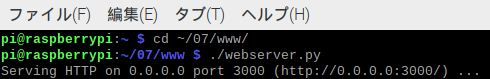
\includegraphics[width=14.986cm]{ome7-img038.png}
\flushleft


\bigskip


\bigskip

3.サーバーが動いているかどうかを確認してみましょう。

\ \ 別のターミナルを立ち上げ、次のコマンドを打ちましょう。

\ \  nmap localhost

\ \ 今回使っているポート番号は:3000です。STATE(状態)がopen(開く)になっています。

\ \ これでサーバーが動いていることが分かります。



\centering
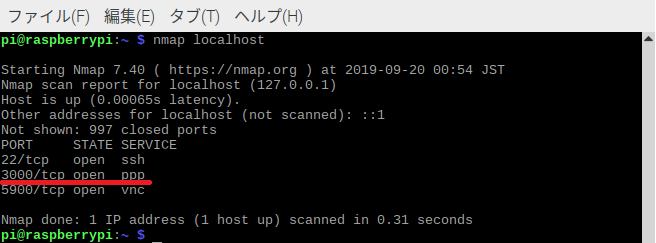
\includegraphics[width=16.124cm]{ome7-img039.png}
\flushleft


\bigskip

4.みなさんが作ったウェブページを表示してみましょう。

\ \ みなさんが作ったindex.htmlの場所はwebserver.pyを起動したディレクトリと同じでしたね。「2」で説明したドキュメントルートです。

\ \ これはwebserver.pyを起動したディレクトリ

\ \  {\textasciitilde}/07/www/

\ \ を指しています。


\bigskip

\ \ 次にブラウザのアドレスバーに打つURLはどのように書けばいいのでしょうか。

\ \ URLの書き方は次のようになります。

\ \ なので自分のパソコンのサーバーを見るには

\centering

\includegraphics[width=13.894cm]{ome7-img040.png}
\flushleft

\ \  \url{http://localhost:3000/}

\ \ というURLになります。

\ \ サーバー名の後の/(スラッシュ)はドキュメントルートを示しています。

\ \ ブラウザはファイル名を指定しないとindex.htmlというファイルを開くように\ruby{設定}{せってい}されて\ \ います。

\ \  \url{http://localhost:3000/}

\ \ をブラウザのアドレスバーに打ってみましょう。

\ \ みなさんが作ったウェブページのHTMLが表示されましたね。

\ \ これは

\ \  \url{http://localhost:3000/index.html}

\ \ と入力しているのと同じことです。



\centering
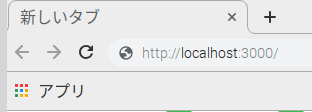
\includegraphics[width=9.551cm]{ome7-img041.png}
\flushleft


\bigskip


\bigskip


\bigskip

\refstepcounter{Exercise}
\clearpage\subsection*{2−3 \theExercise 友だちのホームページを見てみよう}


\centering
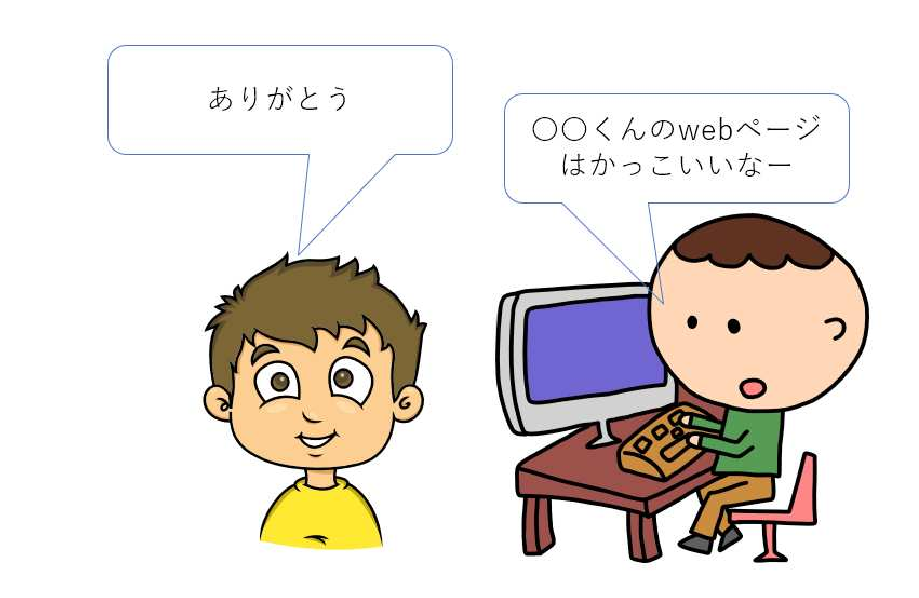
\includegraphics[width=10.423cm]{ome7-img042}
\flushleft


\bigskip



1.
\ruby{左隣}{ひだりどなり}の友達のIPアドレスを確認しよう。

\ \ 友達のターミナルで次のコマンドをうってもらいましょう。

\ \ hostname -I

\ \ そのIPアドレスをメモしましょう。

\ \ [\underline{    }さんのIP:\underline{              }]


\bigskip

2.友達のウェブページを見て見ましょう。

\ \ 自分のサーバーを見るときは

\ \  \url{http://localhost:3000/}

\ \ でした。localhostというのが自分のサーバーという意味でした。

\ \ 今回は友達のサーバーを見たいのでlocalhostの代わりに友達のIPアドレスを打ちましょう。

\ \  \url{http://xxx.xxx.xxx.xxx:3000/}

\ \ \  \url{http://xxx.xxx.xxx.xxx:3000/index.html}

\ \ をブラウザのアドレスバーに打ってみましょう。

\ \ もし左隣の友達のIPアドレスが192.162.33.5だったら

\ \  \url{http://192.162.33.5:3000/index.html}

\ \ となります。

\ \ 友達のウェブページが表示されたら成功です!


\bigskip


\centering
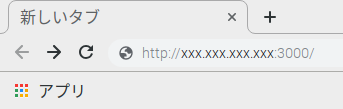
\includegraphics[width=10.659cm]{ome7-img043.png}
\flushleft

\clearpage\subsection*{\bfseries
	注意}

例題7-6の友達のホームページを見てみようでは、以下の図のように同じルータにつながっているラズベリーパイが公開しているホームページは、見ることができます。\ruby{基本}{きほん}同じグループの子たちのホームページは見れるので確認してみてください。

\centering
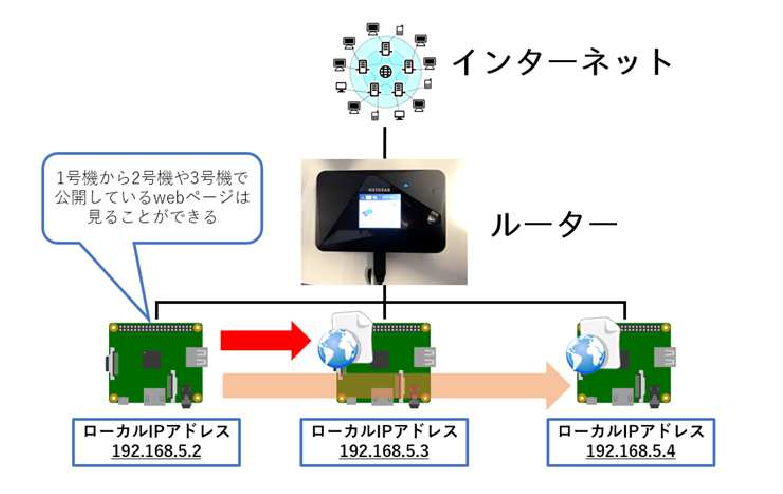
\includegraphics[width=12.284cm]{ome7-img044}
\flushleft


\bigskip


\bigskip



あと、他のルータに接続しているラズベリーパイが公開しているホームページは今回みることができません。実際に試してみても面白いと思います。


\bigskip

\centering
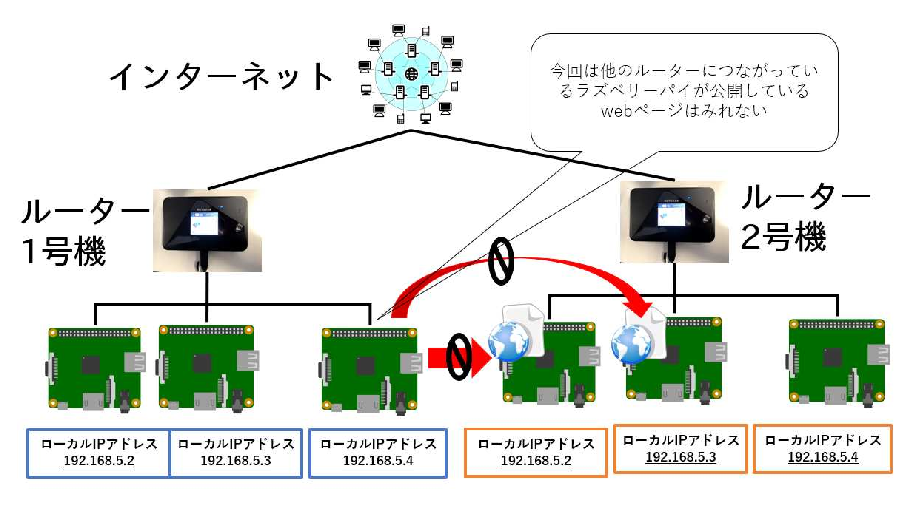
\includegraphics[width=13.166cm]{ome7-img045}
\flushleft


\bigskip


\bigskip

\refstepcounter{Question}\theQuestion 他のグループの友達のホームページを見てみよう、自分とは違うWi-Fiルータに接続している友達のホームページは見れたかどうか答えに書こう



\bigskip

{\bfseries
	\addBlank{答え}}


\bigskip

\if0


	参考 接続できるネットワーク(Wi-Fiルータ)

	NTGR-4643\ \ \ \ パスワード 33995460

	NTGR-3EBC\ \ \ \ パスワード 34986626

	NTGR-3DFC\ \ \ \ パスワード 36976828

\fi

\bigskip


\bigskip

\clearpage\subsection*{3−1 CGIについて勉強しよう}
ここではCGIについて勉強しよう。第1回で作成したwebページはいわば静的なページです。静的なページとは、常に同じ画面を表示するページのことです。ですが、CGI(Common
Gateway
Interface)を用いることによって動きのあるページ、動的なページを作成することができます。動的なページとは表示させるたびに違う画面を表示することができるページのことです。アクセスカウンターはたまにwebページについていることがあります。アクセスカウンタというのは、そのwebページに今までどれぐらいの人がアクセス(接続)したのかを表示させるものです。webページにアクセスするたびにアクセスカウンタの数は\ruby{増}{ふ}えていき、毎回同じ数字にはなりません。これはアクセスするというアクションによってページに変化を起こしているのです。さらにCGIを用いることによって以下の機能を作成することができます。

{\bfseries
・アクセスカウンター}



\centering
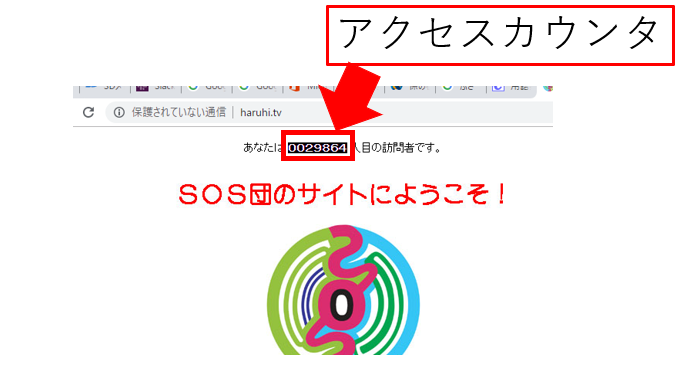
\includegraphics[width=8.176cm]{ome7-img046.png}
\textbf{・アンケートフォーム}\\
\includegraphics[width=6.1cm]{ome7-img047.png}
\flushleft


\bigskip

{\bfseries

	・\ruby{掲示板}{けいじばん}}



\centering
\includegraphics[width=4.431cm]{ome7-img048.png}
\flushleft





\bigskip

みんなが作ったwebページやほかの静的なページはどのようなやり取りで表示させているか見ていきましょう。次の図を見てください。



\bigskip


\centering
\includegraphics[width=13.827cm]{ome7-img049}
\flushleft

\bigskip


webブラウザで検索したりしてwebページを表示させることをリクエスト(要求)といい、そのリクエストを受け取ったそのwebページのあるサーバーが要求したところにレスポンス(返答)を返します。要求されたら返すのみで、webページに変化はなく同じものを見せていました。ですが次の画像をみてください。


\bigskip

\centering
\includegraphics[width=14.065cm]{ome7-img050}
\flushleft

\bigskip


CGIを使った動的ページでは、サーバーが皆さんからwebページを要求されるたびに、CGIプログラムで新しいHTMLを生成しています。それにより、毎回違うwebページを見せることが可能なのです。この教科書では皆さんのラズベリーパイと今までの講義で学んだことを生かしたCGIを体験していきます。


\bigskip

\refstepcounter{Question}\theQuestion 動的なページとはどのようなものでしょうか。また、動的なページを作成する場合に用いるものは何でしょう。


\bigskip

\addBlank{答え}


\bigskip

\addBlank{答え}


\bigskip

\refstepcounter{Exercise}
\clearpage\subsection*{\theExercise CGIを使ってウェブページからLEDをつける}
\addtocounter{Exercise}{-1}\refstepcounter{Exercise}\label{E:CGI}
考え方

まずはラズパイにセンサーボードを取り付けましょう。今回はFaBoは使用しません。

ウェブサーバはウェブブラウザから要求を受けます。”ファイル名.hsp”ファイルへのアクセスをブラウザから行うとサーバはCGIプログラムをサーバ側で起動します。結果はHTMLとしてブラウザ(クライアント)へ返されます。

試しに、CGIプログラムを起動させてみましょう。例題のプログラムはLEDがすでに点灯していれば消灯、消灯してれば点灯するプログラムです。ウェブサーバがウェブブラウザから要求を受けて、CGIプログラムを起動するのでウェブサーバが起動している必要があります。まずはウェブサーバを起動させましょう。

ターミナルを開いて

cd {\textasciitilde}/07/www/

./webserver.py \ \ \ \ で起動できます。

%
%コマンド実行画面
%cd {\textasciitilde}/07/www/
%./webserver.py
%koyaman
%September 20, 2019 2:48 AM


次にウェブブラウザからウェブサーバへCGIの要求を出してみましょう。

ブラウザを開いて、

localhost:3000/cgi-bin/led.hsp

%
%ぶらうざで開いた画面
%koyaman
%September 20, 2019 2:49 AM


\centering
\includegraphics[width=16.574cm]{ome7-img051.png}
\flushleft

にアクセスをしてみましょう。アクセスをすると、プログラムが起動してLEDが点灯します。ブラウザのリロードボタンを押すと消灯します。

\centering
\includegraphics[width=16.166cm]{ome7-img052.png}
\flushleft

cgi-binディレクトリはCGIプログラムを入れるディレクトリです。{\textasciitilde}/07/wwwの下にあります。このディレクトリ内の

”ファイル名”.hsp

はCGIプログラムとして\ruby{扱}{あつ}われます。led.hspはCGIプログラムです。


\bigskip

\clearpage
プログラム解説



\centering
\begin{boxedminipage}{0.95\textwidth}

	\begin{enumerate}
	\setlength{\itemsep}{0cm}
	\item \#include {\textquotedbl}hsp3cl.as{\textquotedbl}

	\item \#include {\textquotedbl}rpz-gpio-cl.as{\textquotedbl}


	\item

	\item mes {\textquotedbl}Content-type: text/html{\textbackslash}n{\textquotedbl}

	\item mes {\textquotedbl}{\textless}html{\textgreater}{\textless}head{\textgreater}{\textless}meta
	charset={\textbackslash}{\textquotedbl}utf-8{\textbackslash}{\textquotedbl}{\textgreater}{\textless}/head{\textgreater}{\textless}body{\textgreater}{\textquotedbl}


	\item

	\item ;現在のGPIO 17の\ruby{値}{あたい}を取得 1 == ON, 0 == OFF

	\item ;CGIからはcgpioinを使う(使い方はgpioinと同じ)

	\item prev\_led = cgpioin(17)

	\item

	\item if prev\_led = 0\{

	\item ;ついていなかった

	\item mes
		{\textquotedbl}{\textless}p{\textgreater}オフでした。つけます{\textless}/p{\textgreater}{\textquotedbl}

	\item next\_led = 1

	\item \}else\{

	\item ;

	\item mes
		{\textquotedbl}{\textless}p{\textgreater}オンでした。けします{\textless}/p{\textgreater}{\textquotedbl}

	\item next\_led = 0

	\item \}

	\item mes {\textquotedbl}{\textless}/body{\textgreater}{\textless}/html{\textgreater}{\textquotedbl}

	\item ;CGIからはcgpioを使う(使い方はgpioと同じ、0以外を書いた場合プログラムが

	\item ;\ruby{終了}{しゅうりょう}してもLEDは点灯し続ける)

	\item cgpio 17, next\_led

	\item end
	\end{enumerate}

\end{boxedminipage}
\flushleft



第3回に使用した命令ではない命令が入っています。\\
詳細はP43に載っています。確認してください。

プログラム解説の3行目

mes {\textquotedbl}Content-type: text/html{\textbackslash}n{\textquotedbl}

はCGIプログラムがウェブサーバに結果を返すときに、結果がHTMLであることを伝えるために必要です。{\textbackslash}nは改行を意味します。本来は改行は2つ必要ですが、mes命令は自動で改行を入れてくれるので、{\textbackslash}nは1つで十分です。


\bigskip
\clearpage
4行目\ruby{以降}{いこう}のmes命令で出力するものは、HTMLの一部として扱われます。

\bigskip

6行目では、文字コードを設定しています。

\bigskip

9行目からLED点灯消灯のプログラムが始まります。

prev\_led = cgpioin(17)

では、GPIO17番の状態を調べています。LEDが点灯していれば1になり、消灯していれば0になります。


\bigskip


10〜17行目では、\ruby{条件}{じょうけん}判断のif文を使って読み取ったLEDの状態を判断します。消灯状態であれば、9行目で

mes
	{\textquotedbl}{\textless}p{\textgreater}オフでした。つけます{\textless}/p{\textgreater}{\textquotedbl}

pタグを使ってメッセージを表示します。

\bigskip

12行目で

next\_led = 1

としてLEDを点灯させるための値を用意します。

\bigskip

消灯以外の状態(つまり点灯状態)の場合は、13行目で

mes
	{\textquotedbl}{\textless}p{\textgreater}オンでした。けします{\textless}/p{\textgreater}{\textquotedbl}

pタグを使ってメッセージを表示します。

\bigskip

18行目で

next\_led = 0

としてLEDを消灯させるための値を用意します

\bigskip

20行目で実際に値をGPIO17へ書き込みます。

cgpio 17, next\_led




\bigskip

21行目の

end

でプログラムの終了をします。


\bigskip



第7回のCGIを使うプログラムでは、第3回の授業とはちがう命令を使います。\\
第3回の命令でCGIを使おうとすると、上手く動かなくなってしまうからです。\\
下の表にそれぞれの命令をまとめておきます。\\

\clearpage
\begin{flushleft}
	\tablefirsthead{}
	\tablehead{}
	\tabletail{}
	\tablelasttail{}
	\begin{supertabular}{|m{5.0cm}|m{5.5cm}|m{7.0cm}|}
		\hline
		第3回に使った
		命令名 &
		CGIを使うときの
		命令名&
		効果
		\\\hline

		\#include “rpz-gpio.as”&
		\#include “rpz-gpio-cl.as”&
		プログラムのはじめに書くことでLED
		の点灯や消灯の命令が使えるようになります。
		\\\hline

		onoff\ = \ gpioin(17)&

		onoff\ = \ cgpioin(17)&
		17番のGPIOのLEDが点灯していれば変数onoffに1が、
		消灯していれば変数onoffに0が入ります。
		17をほかの番号に変えることで、
		ほかのLEDの状態を確認できます。
		\\\hline

		gpio \ 18,\ 1&
		cgpioin \ 18,\ 1&
		18番のGPIOのLEDを点灯します。
		1を0にすると消灯になります。
		18をほかの番号に変えることで、
		ほかのLEDを点灯、消灯できます。
		\\\hline



	\end{supertabular}
\end{flushleft}






\bigskip


\bigskip
\refstepcounter{Question}\theQuestion

{\bfseries
	友達のLEDをCGIで点灯させてみよう。}

{\bfseries

	点灯、消灯時のウェブページに表示されるメッセージを\ruby{変更}{へんこう}してみよう。}

{\bfseries
	他の色のLEDも点灯、消灯できるようにしよう。}

{\bfseries
	Faboのセンサ(LED,
	\ruby{振動子}{しんどうし}などのデジタルセンサ)を接続してCGIから動かせるようにしてみよう。}


\bigskip

\refstepcounter{Exercise}
\clearpage\subsection*{\theExercise URLを使ってCGIに情報を\ruby{渡}{わた}す}
\addtocounter{Exercise}{-1}\refstepcounter{Exercise}\label{E:URL}
考え方

CGIのプログラムに情報を渡すことができればより便利なプログラムが作れます。ここでは\ruby{単純}{たんじゅん}なURLを用いた方法を使います。URLに\ruby{埋}{う}め込まれた情報はクエリストリングと呼ばれます。クエリストリングはまずウェブサーバへ送られ、ウェブサーバがCGIプログラムへクエリストリングを渡します。これによりCGIプログラムはURLに埋め込まれた情報を扱うことができます。


\bigskip

まずは、ブラウザを開いて、

localhost:3000/cgi-bin/querystring.hsp?msg=helloworld

を入力してみましょう。

%
%ぶらうざで開いた画面
%helloworldと表示されている
%koyaman
%September 20, 2019 2:49 AM


画面にhelloworldと表示されたと思います。



\centering
\includegraphics[width=15.528cm]{ome7-img053.png}
\flushleft

localhost:3000/cgi-bin/querystring.hsp?msg=goodbye

に変更してみてください。

%
%ぶらうざで開いた画面
%goodbyeと表示されている
%koyaman
%September 20, 2019 2:49 AM


次はgoodbyeと表示されたと思います。

\centering
\includegraphics[width=15.494cm]{ome7-img054.png}
\flushleft

このようにURLに情報を埋め込んでおくことでCGIのプログラムはこれを受け取り処理をすることができます。URLに埋め込まれた情報はクエリストリングと呼ばれます。この情報はまずウェブサーバが受け取ります。ウェブサーバは少し\ruby{処理}{しょり}をしてCGIプログラムへ渡します。

クエリストリングはURLの最後に?をつけて始めます。

クエリストリングの形は

名前=値

のようになっています。この例では

msg=helloworld

msg=goodbye

などとなっています。これはmsgという名前の値はhelloworld,
goodbyeであることを意味します。HSPの変数と同じような感じです。

次にCGIプログラムでどのようにクエリストリングを扱っているのか見てみましょう。


\bigskip

プログラム解説



\centering
\begin{boxedminipage}{16.233cm}
	\#include {\textquotedbl}hsp3cl.as{\textquotedbl}

	\#include {\textquotedbl}cgi.as{\textquotedbl}

	mes {\textquotedbl}Content-type: text/html{\textbackslash}n{\textquotedbl}

	mes {\textquotedbl}{\textless}html{\textgreater}{\textless}head{\textgreater}{\textless}meta
	charset={\textbackslash}{\textquotedbl}utf-8{\textbackslash}{\textquotedbl}{\textgreater}{\textless}/head{\textgreater}{\textless}body{\textgreater}{\textquotedbl}

	getqueryval {\textquotedbl}msg{\textquotedbl}, q

	mes q

	mes {\textquotedbl}{\textless}/body{\textgreater}{\textless}/html{\textgreater}{\textquotedbl}

	end
\end{boxedminipage}
\flushleft


\bigskip


\bigskip

5行目の

getqueryval “msg”, q

はクエリストリング内の名前が”msg”に対応する値を変数qに入れています。

localhost:3000/cgi-bin/querystring.hsp?msg=helloworld

というURLがあった場合、

変数qにはhelloworldが文字列として入ります。

6行目で表示をしています。

このように\ruby{簡単}{かんたん}にプログラムでクエリストリングを受け取ることができます。クエリストリングが使えると、{\textless}form{\textgreater}{\textless}/form{\textgreater}を使ってCGIに処理を\ruby{依頼}{いらい}できたり、CGIの処理をより高度にすることができます。次の例では、クエリストリングを使ってLEDを点灯消灯します。

ほとんどのウェブサイトは検索をするさいにURLに検索ワードを埋め込んでいます。


\bigskip

\refstepcounter{Question}\theQuestion 画面に”ありがとう”と表示させよう。

	\refstepcounter{Exercise}
\clearpage\subsection*{\theExercise クエリストリングを使ってLEDを操作する}
\addtocounter{Exercise}{-1}\refstepcounter{Exercise}\label{E:QS}
この例では、クエリストリングを使ってLEDを点灯消灯させてみましょう。


\bigskip

まずは、ブラウザを開いて、

localhost:3000/cgi-bin/qsled.hsp?led=17\&val=1

を入力してみましょう。

%
%ぶらうざで開いた開いた画面
%koyaman
%September 20, 2019 2:50 AM


\centering
\includegraphics[width=17.006cm]{ome7-img055.png}
\flushleft

実行するとLED17が光ります。val=1をval=0にすると消えます。URLに埋め込まれた情報をもとにCGIプログラムはLEDを操作していることがわかります。URLに埋め込まれた情報はクエリストリングと呼ばれます。


\bigskip

クエリストリングを\ruby{詳}{くわ}しく見てみましょう。

クエリストリングとはURLの最後に?をつけて始めます。?のあとには

名前(変数名みたいなもの) = 値

の形を続けます。例えば、

localhost:3000/cgi-bin/qsled.hsp?led=17

のようにかけます。この場合は、

名前がled、値が17となります。

複数の情報を渡したい場合は\&を使います。

localhost:3000/cgi-bin/qsled.hsp?led=17\&val=1

のようになります。

名前1がled、値1が17となり

名前2がval、値2が1となります。

このクエリストリングをプログラムから扱う方法を次に学びましょう。

\clearpage
プログラム解説



\centering
\begin{boxedminipage}{16.538cm}
	\#include {\textquotedbl}hsp3cl.as{\textquotedbl}

	\#include {\textquotedbl}rpz-gpio-cl.as{\textquotedbl}

	\#include {\textquotedbl}cgi.as{\textquotedbl}

	mes {\textquotedbl}Content-type: text/html{\textbackslash}n{\textquotedbl}

	mes {\textquotedbl}{\textless}html{\textgreater}{\textless}head{\textgreater}{\textless}meta
	charset={\textbackslash}{\textquotedbl}utf-8{\textbackslash}{\textquotedbl}{\textgreater}{\textless}/head{\textgreater}{\textless}body{\textgreater}{\textquotedbl}


	\bigskip

	;
	クエリストリングからledを探して、値をled\_portへ入れる

	getqueryval {\textquotedbl}led{\textquotedbl}, led\_port

	;
	クエリストリングからvalを探して、値をled\_valへ入れる

	getqueryval {\textquotedbl}val{\textquotedbl}, led\_val

	;文字列なので数値へ変換する

	led\_port = int(led\_port)

	led\_val = int(led\_val)


	\bigskip

	;
	点灯消灯を判断して、メッセージをpタグで表示する

	if(led\_val = 1) \{

	\ \ \ \ mes {\textquotedbl}{\textless}p{\textgreater}GPIO{\textquotedbl} + led\_port +
	{\textquotedbl}を点灯します{\textless}/p{\textgreater}{\textquotedbl}

	\} else \{

	\ \ \ \ mes {\textquotedbl}{\textless}p{\textgreater}GPIO{\textquotedbl} + led\_port +
	{\textquotedbl}を消灯します{\textless}/p{\textgreater}{\textquotedbl}

	\}


	\bigskip

	;
	クエリストリングのledで指定されたGPIOにvalで指定された値を書き込む

	; localhost:3000/cgi-bin/qsled.hsp?led=17\&val=1

	; の場合、LED17を点灯させる

	cgpio led\_port, led\_val

	mes {\textquotedbl}{\textless}/body{\textgreater}{\textless}/html{\textgreater}{\textquotedbl}

	end
\end{boxedminipage}
\flushleft

\bigskip



\bigskip


\bigskip

8行目、10行目で使用している

getqueryval命令でクエリストリングを受け取ります。この命令は

getqueryval 名前, 値を入れる変数

のように使います。クエリストリングから名前を探して、変数へ値を文字列としていれます。

例えば、

getqueryval led, led\_port

の場合にlocalhost:3000/cgi-bin/qsled.hsp?led=17

とクエリストリングを与えたとすると、

led\_portには17が入ります。

12,13行目で

文字列から数値へ変換しています。

16〜20行目では、点灯するのか消灯するのかを条件判断を使って判断しています。led\_valが1のとき(val=1がクエリストリングで与えられたとき)に点灯する、その他のときは消灯するとします。

25行目で実際に点灯、消灯を行います。

cgpio命令は数値でGPIO番号、オンオフ(1,0)を受け付けるので、文字列から変換をしました。


\bigskip

\refstepcounter{Question}\theQuestion

{\bfseries
	GPIO17以外のLEDを光らせてみよう。}


\bigskip


\bigskip

\refstepcounter{Exercise}
\clearpage\subsection*{\theExercise CGIを使ってOpenJtalkに読み上げをさせよう}
\addtocounter{Exercise}{-1}\refstepcounter{Exercise}\label{E:Jtalk}
考え方

ウェブページから読み上げさせたい文章を受け取って、OpenJtalkにCGIから読み上げをさせよう。

まずは、試してみよう。

ブラウザを開いて

localhost:3000/jtalk.html

にアクセスをしてみよう。

%
%ぶらうざで開いた画面n
%koyaman
%September 20, 2019 2:50 AM


\centering
\includegraphics[width=14.319cm]{ome7-img056.png}
\flushleft

テキストボックスに読み上げさせたい文章を入れて送信をしてみよう。送信を押すとCGIプログラムへ文章が送られ、OpenJtalkで音声合成をします。


\bigskip

結果をウェブページのaudioタグ(音声を再生するタグ)へ渡して\ruby{再生}{さいせい}をします。

%
%
%音声ファイルを再生する画面のスクショ
%koyaman
%September 20, 2019 2:50 AM


\centering
\includegraphics[width=14.392cm]{ome7-img057.png}
\flushleft

\clearpage
プログラム解説

{\textasciitilde}/07/www/jtalk.html



\centering
\begin{boxedminipage}{16.148cm}
	{\textless}!DOCTYPE html{\textgreater}

		{\textless}html{\textgreater}

	{\textless}head{\textgreater}

	\ \ \ \ {\textless}meta charset={\textquotedbl}utf-8{\textquotedbl}{\textgreater}

	{\textless}/head{\textgreater}

	{\textless}body{\textgreater}

	\ \ \ \ {\textless}form action={\textquotedbl}cgi-bin/jtalk.hsp{\textquotedbl}
	method={\textquotedbl}GET{\textquotedbl}{\textgreater}

	\ \ \ \ \ \ \ \ {\textless}input type={\textquotedbl}text{\textquotedbl}
	name={\textquotedbl}sentence{\textquotedbl}{\textgreater}

	\ \ \ \ \ \ \ \ {\textless}input type={\textquotedbl}submit{\textquotedbl}
	value={\textquotedbl}送信{\textquotedbl}{\textgreater}

	\ \ \ \ \ \ \ \ {\textless}input type={\textquotedbl}reset{\textquotedbl}
	value={\textquotedbl}リセット{\textquotedbl}{\textgreater}

	\ \ \ \ {\textless}/form{\textgreater}

	{\textless}/body{\textgreater}

	{\textless}/html{\textgreater}
\end{boxedminipage}
\flushleft
\bigskip


\bigskip


\bigskip



\bigskip

7〜11行目では、CGIようにフォーム(form)を用意しています。

文字を入れるテキストボックスが一つと送信用のボタンが一つ、テキストボックスをリセットするボタンが一つあります。

%
%スクリーンショット
%ブラウザでjtalk.htmlを開いた画像
%koyaman
%September 19, 2019 11:59 PM


7行目の

{\textless}form action={\textquotedbl}cgi-bin/jtalk.hsp{\textquotedbl}
method={\textquotedbl}GET{\textquotedbl}{\textgreater}

action=”cgi-bin/jtalk.hsp”

はフォームに入力された情報をを受ける(処理する)CGIプログラムを指定します。

method=”GET”

はクエリストリングとしてフォームの情報をCGIに渡すことを指示しています。

8行目の

{\textless}input type={\textquotedbl}text{\textquotedbl} name={\textquotedbl}sentence{\textquotedbl}{\textgreater}

では、テキストボックスを作っています。

name=”sentence”

はクエリストリングの名前を指定します。入力された文字列が値となります。ちなみにsentenceとは日本語にすると”文章”という意味になります。

例えば、テキストボックスに

“こんにちは”とテキストボックスに入力され、送信された場合

\clearpage
\bigskip



\centering
\includegraphics[width=14.392cm]{ome7-img057.png}

\centering
\includegraphics[width=14.319cm]{ome7-img056.png}
\flushleft


\bigskip

%
%スクショ
%こんにちはとテキストボックスに
%koyaman
%September 20, 2019 12:04 AM


ウェブサーバにこのような要求を出します。

IPアドレス:3000/cgi-bin/jtalk.hsp?sentence=こんにちは

実際には”こんにちは”という文字列はURL内ではある\ruby{規則}{きそく}に\ruby{沿}{そ}って記号、数値に変換されています。

このことをパーセントエンコーディングといいます。CGIプログラムにクエリストリングが渡される前にウェブサーバは記号、数値に変換された文字列をもとに戻します。よって、プログラム内では入力された文字列と同じものを扱うことができます。

{\textasciitilde}/07/www/cgi-bin/jtalk.hsp

\centering
\begin{boxedminipage}{\textwidth}
	\#include {\textquotedbl}hsp3cl.as{\textquotedbl}

	\#include {\textquotedbl}jtalk.as{\textquotedbl}

	\#include {\textquotedbl}cgi.as{\textquotedbl}


	\bigskip

	mes {\textquotedbl}Content-type: text/html{\textbackslash}n{\textquotedbl}

	mes {\textquotedbl}{\textless}html{\textgreater}{\textless}head{\textgreater}{\textless}meta
	charset={\textbackslash}{\textquotedbl}utf-8{\textbackslash}{\textquotedbl}{\textgreater}{\textless}/head{\textgreater}{\textless}body{\textgreater}{\textquotedbl}


	\bigskip

	getqueryval {\textquotedbl}sentence{\textquotedbl}, sentence

	jtsave sentence, wav\_file

	mes {\textquotedbl}{\textless}p{\textgreater}{\textquotedbl} + sentence +
	{\textquotedbl}{\textless}/p{\textgreater}{\textquotedbl}


	\bigskip

	mes {\textquotedbl}{\textless}audio src={\textbackslash}{\textquotedbl}{\textquotedbl} \ + wav\_file +
	{\textquotedbl}{\textbackslash}{\textquotedbl}
	type={\textbackslash}{\textquotedbl}audio/wav{\textbackslash}{\textquotedbl} controls{\textgreater}{\textquotedbl}

	mes {\textquotedbl}{\textless}/body{\textgreater}{\textless}/html{\textgreater}{\textquotedbl}

	end
\end{boxedminipage}
\flushleft

\bigskip

8行目でjtalk.htmlのフォームの

{\textless}input type={\textquotedbl}text{\textquotedbl} name={\textquotedbl}sentence{\textquotedbl}{\textgreater}

に入っている値を取り出しています。取り出した値はsentence変数へ入れています。

9行目の

jtsave sentence, wav\_file

はsentence変数の中の文字列を音声合成して音声ファイルのファイル名をwav\_file変数へ入れています。

12行目の

mes {\textquotedbl}{\textless}audio src={\textbackslash}{\textquotedbl}{\textquotedbl} \ + wav\_file +
{\textquotedbl}{\textbackslash}{\textquotedbl}
type={\textbackslash}{\textquotedbl}audio/wav{\textbackslash}{\textquotedbl} controls{\textgreater}{\textquotedbl}

	{\textless}audio{\textgreater}タグは音声ファイルを再生することができます。

src=”ファイル名”

では、再生するファイルを指定します。指定するファイルはドキュメントルート以下にないといけません。つまり、ドキュメントルートである{\textasciitilde}/07/wwwの中にある必要があります。

jtsave命令で作った音声ファイルは{\textasciitilde}/07/www/tmpの中にあります。ファイル名はwav\_file変数に入っています。

“
“の中で”を使うには{\textbackslash}”のように書きます。

type=”audio/wav”

では、音声ファイルの種類を決めます。jtsave命令が作る音声ファイルの場合は、

type=”audio/wav”にします。

controlsをつけると、再生ボタン、ミュートボタンなどが表示されます。

再生ボタンを押すと音声合成した音声ファイルが再生されます。

\clearpage
\refstepcounter{Question}\theQuestion

{\bfseries
	”おはようございます””こんばんは””ありがとうございます”を読ませてみよう。}


\bigskip

できる人は自分の自己紹介ページに({\textasciitilde}/07/www/index.html)に作ったフォームを変更して、こちらからCGIプログラムを起動するようにしましょう。

\ HINT: jtalk.htmlを参考にしてください。

\refstepcounter{Exercise}
\clearpage\subsection*{\theExercise CGIでセンサーの情報を表示させる}
\addtocounter{Exercise}{-1}\refstepcounter{Exercise}\label{E:Sensors}
考え方

温度、温度、\ruby{気圧}{きあつ}、照度センサーの情報をCGIを使ってウェブページから見れるようにしましょう。


\bigskip

まずは、プログラム実行してみましょう。

ブラウザを開いて、

localhost:3000/cgi-bin/sensors.hsp

にアクセスしてください。


%
%スクショ
%ブラウザで開いたときの
%koyaman
%September 20, 2019 2:37 AM


\centering
\includegraphics[width=17.0cm]{ome7-img058.png}
\flushleft


\bigskip

温度センサーの値が表示されていると思います。

リロードするたびに値が更新されます。

今は温度センサーしか表示をしていないので、他のセンサーの値も表示させるように変更してみましょう。

%
%その他のセンサーを表示させた完成図のスクショ
%koyaman
%September 20, 2019 2:45 AM


\centering
\includegraphics[width=12.34cm]{ome7-img059.png}
\flushleft

次にプログラムを見てみましょう。


\clearpage
プログラム解説



\centering
\begin{boxedminipage}{16.81cm}
	\#include {\textquotedbl}rpz-gpio-cl.as{\textquotedbl}

	\#include {\textquotedbl}hsp3cl.as{\textquotedbl}


	\bigskip

	mes {\textquotedbl}Content-type: text/html{\textbackslash}n{\textquotedbl}

	mes {\textquotedbl}{\textless}html{\textgreater}{\textless}head{\textgreater}{\textless}meta
	charset={\textbackslash}{\textquotedbl}utf-8{\textbackslash}{\textquotedbl}{\textgreater}{\textless}/head{\textgreater}{\textless}body{\textgreater}{\textquotedbl}


	\bigskip

	i2c\_ch\_bme\ = \ 0\\
	i2c\_ch\_tsl \ = \ 1

	\bigskip

	fail \ = \ init\_bme(i2c\_ch\_bme)\ \ \ \ ; 温\ruby{湿}{しつ}度気圧センサ bm280
	を初期化する

	if fail \{\ \ \ \ \ \ \ \ \ \ \ \   ; 初期化成功チェック

	\ \ mes {\textquotedbl}failed to init bme: {\textquotedbl} + fail

	\ \ end

	\}


	\bigskip

	init\_lux i2c\_ch\_tsl\ \ \ \ \ \ ; 照度センサ
	tsl2572を初期化する


	\bigskip

	*main


	\bigskip

	\ \ temp = get\_temp(i2c\_ch\_bme)\ \ \ \ ; 温度取得\\
	\ \ hum \ = get\_hum(i2c\_ch\_bme)\ \ \ \ ; 湿度取得\\
	\ \ press= get\_press(i2c\_ch\_bme)\ \ \ \ ; 気圧取得\\
	\ \ lux \ = get\_lux(i2c\_ch\_bme)\ \ \ \ ; 照度取得\\


	\bigskip


	\bigskip

	\ \ ; 取得したデータの表示

	\ \ mes {\textquotedbl}{\textless}p{\textgreater}温度 : {\textquotedbl} + temp + {\textquotedbl}
	[℃]{\textless}/p{\textgreater}{\textquotedbl}


	\bigskip

	\ \ \ \ mes {\textquotedbl}{\textless}/body{\textgreater}{\textless}/html{\textgreater}{\textquotedbl}

	\ \ \ \ end
\end{boxedminipage}
\flushleft
この例題は{\textasciitilde}/03/sensors.hspをもとにしています。詳しい解説はそちらを参照してください。

20~23行目で温度、湿度、気圧、照度センサーから情報を取得しています。

結果はそれぞれtemp, hum, press,
lux変数へ入っています。

27行目で、温度センサーの値をpタグで表示しています。

\bigskip


\bigskip


\bigskip

\clearpage
\refstepcounter{Question}\theQuestion

友達のCGIへアクセスして、センサーの値を確認してみよう。

温度センサーと同様に、湿度、気圧、照度センサーの値も表示させてみましょう。

\begin{center}
	\begin{boxedminipage}{0.5\textwidth}
		localhost:3000/cgi-bin/sensors\_table.hsp
	\end{boxedminipage}
\end{center}

にブラウザでアクセスをしてみましょう。

温度センサーの値が表形式で表示されたと思います。

%
%スクショ
%実行画面
%localhost:3000/cgi{}-bin/sensors\_table.hsp
%koyaman
%September 20, 2019 2:44 AM


\centering
\includegraphics[width=16.9cm]{ome7-img060.png}
\flushleft

次は、湿度、気圧、照度センサーの値を表形式で表示するように変更してみましょう。

\refstepcounter{Exercise}
\clearpage\subsection*{\theExercise 赤外線をウェブページから送信する}
\addtocounter{Exercise}{-1}\refstepcounter{Exercise}\label{E:IR}
CGIを使ってウェブページから赤外線を送信できるようにしましょう。

まずは、サンプルを動かしてみましょう。

ウェブブラウザを開いて

localhost:3000/ir.html

を開きましょう。

%
%開いた画像
%
%koyaman
%September 20, 2019 4:01 AM


\centering
\includegraphics[width=17.006cm]{ome7-img061.png}
\flushleft

ボタンを押すとCGIで赤外線の送信をするコマンドが実行されます。

コマンドは、

irsend SEND\_ONCE fan onoff

が実行されます。リモコンの名前はfan、信号の名前はonoffになっています。

リモコンの名前、信号の名前が違う場合は、

{\textasciitilde}/07/www/cgi-bin/ir.hsp

を開いて

exec “irsend SEND\_ONCE fan onoff”

を変更して保存しましょう。

同じ場合はそのままで\ruby{大丈夫}{だいじょうぶ}です。

%
%スクショ
%ir.htmlのボタン
%koyaman
%September 20, 2019 4:05 AM


\centering
\includegraphics[width=16.671cm]{ome7-img062.png}
\flushleft

ブラウザのファン\ruby{電源}{でんげん}ボタンを押すと、CGIが起動して

赤外線を送信します。


\bigskip

\clearpage
プログラム解説

{\textasciitilde}/07/www/ir.html

8行目でフォームの\ruby{内容}{ないよう}を受け取るCGIを設定しています。

\centering
\begin{boxedminipage}{0.95\textwidth}
	{\textless}!DOCTYPE html{\textgreater}

		{\textless}html{\textgreater}

	{\textless}head{\textgreater}

	\ \ \ \ {\textless}meta charset={\textquotedbl}utf-8{\textquotedbl}{\textgreater}

	{\textless}/head{\textgreater}

	{\textless}body{\textgreater}

	\ \ \ \ {\textless}h2{\textgreater}赤外線リモコン{\textless}/h2{\textgreater}

	\ \ \ \ {\textless}form action={\textquotedbl}cgi-bin/ir.hsp{\textquotedbl}
	method={\textquotedbl}GET{\textquotedbl}{\textgreater}

	\ \ \ \ \ \ \ \ {\textless}p{\textgreater}

	\ \ \ \ \ \ \ \ \ \ \ \ ファン電源 : {\textless}input type={\textquotedbl}submit{\textquotedbl}
	value={\textquotedbl}power{\textquotedbl} name={\textquotedbl}command{\textquotedbl}{\textgreater}

	\ \ \ \ \ \ \ \ {\textless}/p{\textgreater}

	\ \ \ \ {\textless}/form{\textgreater}

	{\textless}/body{\textgreater}

	{\textless}/html{\textgreater}
\end{boxedminipage}
\flushleft
{\textasciitilde}/07/www/cgi-bin/ir.hsp

がCGIとしてに起動します。

10行目で送信ボタンを作っています。

{\textless}input type={\textquotedbl}submit{\textquotedbl} value={\textquotedbl}power{\textquotedbl}
name={\textquotedbl}command{\textquotedbl}{\textgreater}

クエリストリングの名前はcommandで値はpowerとなります。このボタンが押されるとCGIが起動します。


\bigskip


\bigskip

\bigskip



\centering
\begin{boxedminipage}{16.36cm}
	\#include {\textquotedbl}hsp3cl.as{\textquotedbl}

	\#include {\textquotedbl}cmdexec.as{\textquotedbl}

	\#include {\textquotedbl}cgi.as{\textquotedbl}


	\bigskip

	mes {\textquotedbl}Content-type: text/html{\textbackslash}n{\textquotedbl}

	mes {\textquotedbl}{\textless}html{\textgreater}{\textless}head{\textgreater}{\textless}meta
	charset={\textbackslash}{\textquotedbl}utf-8{\textbackslash}{\textquotedbl}{\textgreater}{\textless}/head{\textgreater}{\textless}body{\textgreater}{\textquotedbl}


	\bigskip

	getqueryval {\textquotedbl}command{\textquotedbl}, cmd

	if cmd = {\textquotedbl}power{\textquotedbl} \{

	\ \ mes
		{\textquotedbl}{\textless}p{\textgreater}ファンの電源をおします。{\textless}/p{\textgreater}{\textquotedbl}

	\ \ exec {\textquotedbl}irsend SEND\_ONCE fan onoff{\textquotedbl}

	\} else \{

	\ \ \ \ mes
		{\textquotedbl}{\textless}p{\textgreater}コマンドが正しくありません{\textless}/p{\textgreater}{\textquotedbl}

	\ \ \ \ mes {\textquotedbl}{\textless}p{\textgreater}{\textquotedbl} + cmd +
	{\textquotedbl}{\textless}/p{\textgreater}{\textquotedbl}

	\}


	\bigskip

	mes {\textquotedbl}{\textless}/body{\textgreater}{\textless}/html{\textgreater}{\textquotedbl}

	end
\end{boxedminipage}
\flushleft

\bigskip




\bigskip


\bigskip

8行目でクエリストリングから名前がcommandに対応する値を取り出してcmd変数へ入れています。

9〜15行目で受け取ったcmd変数をもとに条件判断をしています。cmdがpowerのときにファンの電源をつける赤外線を送っています。

それ以外の場合は正しいコマンドでないとして、メッセージを表示しています。


\bigskip

\bigskip
\refstepcounter{Question}\theQuestion

ファンの電源をつける以外の赤外線送信機能を追加してみよう。

\ \ HINT :
まずは、ir.htmlにボタンを追加しよう。

\ \ \ \ そのあと、ir.hspの条件判断を追加しよう。

ir.htmlのフォームを自己紹介ページの一番下に付け加えよう。


\bigskip


\bigskip


\clearpage
CGIを使うときに便利なHSPの命令一覧

\begin{flushleft}
	\tablefirsthead{}
	\tablehead{}
	\tabletail{}
	\tablelasttail{}
	\begin{supertabular}{|m{5.467cm}|m{3.181cm}|m{7.7cm}|}
		\hline
		命令名/使い方 &
		例題 &
		効果\\\hline
		\#include “cgi.as”

		getqueryval “name”, var &
		\ref*{E:URL}

		\ref*{E:QS}

		\ref*{E:Jtalk}

		\ref*{E:IR} &
		クエリストリングから名前”name”を探して文字列として値を変数varへ入れる。

		\textbf{localhost:3000/cgi-bin/querystring.hsp?name=val}
		の場合、
		varにはvalが入る。\\\hline

		\#include “rpz-gpio-cl.as”
		cgpio 17, 1&
		\ref*{E:CGI}

		\ref*{E:QS}

		\ref*{E:Sensors} &
		gpio 命令と使い方は同じ。GPIO17 番に 1 を
		書き込む。gpio 命令との違いはプログラム終
		了時にも書き込んだ値が持続する。例えば、
		cgpio 17, 1 を実行すると、
		プログラム終了時でも 17 番の GPIO は 1 の
		ままになる。\\\hline

		\#include “rpz-gpio-cl.as”
		onoff = cgpioin(17)&
		\ref*{E:CGI} &
		gpio 命令と同じ。cgpio でプログラム終了時
		でも効果を持続させたい場合はこちらを使用
		する必要がある。\\\hline

		\#include “rpz-gpio-cl.as”&
		\ref*{E:CGI}

		\ref*{E:QS}

		\ref*{E:Sensors} &
		\#include “rpz-gpio.as”のコマンドライン\ruby{版}{ばん}
		コマンドラインや CGI で動くプログラムを書
		く場合はこちらを使う。cgpio, cgpioin 命令
		以外は同じ命令が使える。\\\hline

		\#include “jtalk.as”

		jtsave “こんにちは”, hello &
		\ref*{E:Jtalk} &
		“こんにちは”をOpenJtalkで音声合成をして、作った音声ファイルのファイル名をhello変数へ入れる。音声ファイルは/tmp/ディレクトリの下にランダムなファイル名で入る。

		例えば、hello変数の中身は

		“/tmp/tmp.abzgda”のような感じになる。 \\\hline
		end &
		すべての例題 &
		プログラムの終了を意味する。この命令はCGI用のプログラムを終了するときに必要。この命令がないとCGIのプログラムは終了しない。(ブラウザの読み込みが終わらなくなる。)\\\hline
	\end{supertabular}
\end{flushleft}

\bigskip

{\bfseries
	付録 ウェブサーバの停止方法}

電源を切る前、ウェブサーバが起動しているターミナルを\ruby{閉}{と}じる前、ウェブサーバを停止したいときは、ウェブサーバを起動したターミナル(./webserver.pyを実行している画面)を選択して


\bigskip

CtrlとCを同時に押します。


\bigskip

それでウェブサーバは終了します。


\bigskip


\bigskip


\bigskip

\end{document}
